\pSpace Στο παρόν κεφάλαιο παρουσιάζεται ένα εγχειρίδιο χρήσης για όλες τις διαθέσιμες σελίδες της εφαρμογής. Χωρίζεται σε τρία μέρη: αρχική σελίδα, εγγραφή/ταυτοποίηση και \e{iPM}. Η κάθε ενότητα περιέχει περιγραφή, οδηγίες και εικόνες που αφορούν την συγκεκριμένη σελίδα η λειτουργία.\\
\pSpace Επίσης το τρίτο μέρος που αφορά το \e{iPM}, χωρίζεται σε δύο ενότητες, \e{user} και \e{project}. Το πρώτο εξηγεί τις ενέργειες του χρήστη ως προς το προσωπικό \e{Dashboard, Profile} κλπ, ενώ στο δεύτερο τις ενέργειες που μπορούν να συμβόυν σε ένα έργο.\\
\section{\e{Homepage}}
\pSpace Η αρχική σελίδα (βλ. σχ. \ref{fig:homepage}) έχει τον ρόλο ενός \e{landing page}, δηλαδή η σελίδα που θα πρωτοσυναντήσει ο χρήστης όταν αποκτήσει πρόσβαση στην διεύθυνση της εφαρμογής (\e{\url{https://pmthesis.herokuapp.com}}).\\
\pSpace Χρησιμοποιώντας το μενού που βρίσκεται στον επάνω μέρος της σελίδας, ο χρήστης μπορεί να μετακινηθεί στην ενότητα που τον εδνιαφέρει χωρίς περαιτέρων αλληλεπιδράσεις.\\
\pSpace Στην ενότητα \e{Authenticate}, έχει δύο επιλογές για να αποκτήσει πρόσβαση στην εφαρμογή: εγγραφή η σύνδεση με ένα υπαρκτό λογαριασμό. Η πρώτη τον οδηγεί στην διεύθυνση \e{\url{https://pmthesis.herokuapp.com/auth/signup}} ενώ η δεύτερη στην \e{\url{https://pmthesis.herokuapp.com/auth/signin}}.\\
\pSpace Επιπλέον στην τελευταία ενότητα, υπάρχει μια φόρμα επικοινωνίας, που έχει ως στόχο την αποστολή ερωτημάτων, προβλημάτων που αφορούν την εφαρμογή. Ακόμη, στο κάτω μέρος της σελίδας υπάρχουν συντομεύσεις για το \e{repository} στο \e{Github}, για την σελίδα του Τμήματος Πληροφορικής Σερρών και μια ακόμη που αφορά οδηγίες χρήσης εφαρμογής.\\
\pagebreak

\begin{figure}[!htb]
\centering
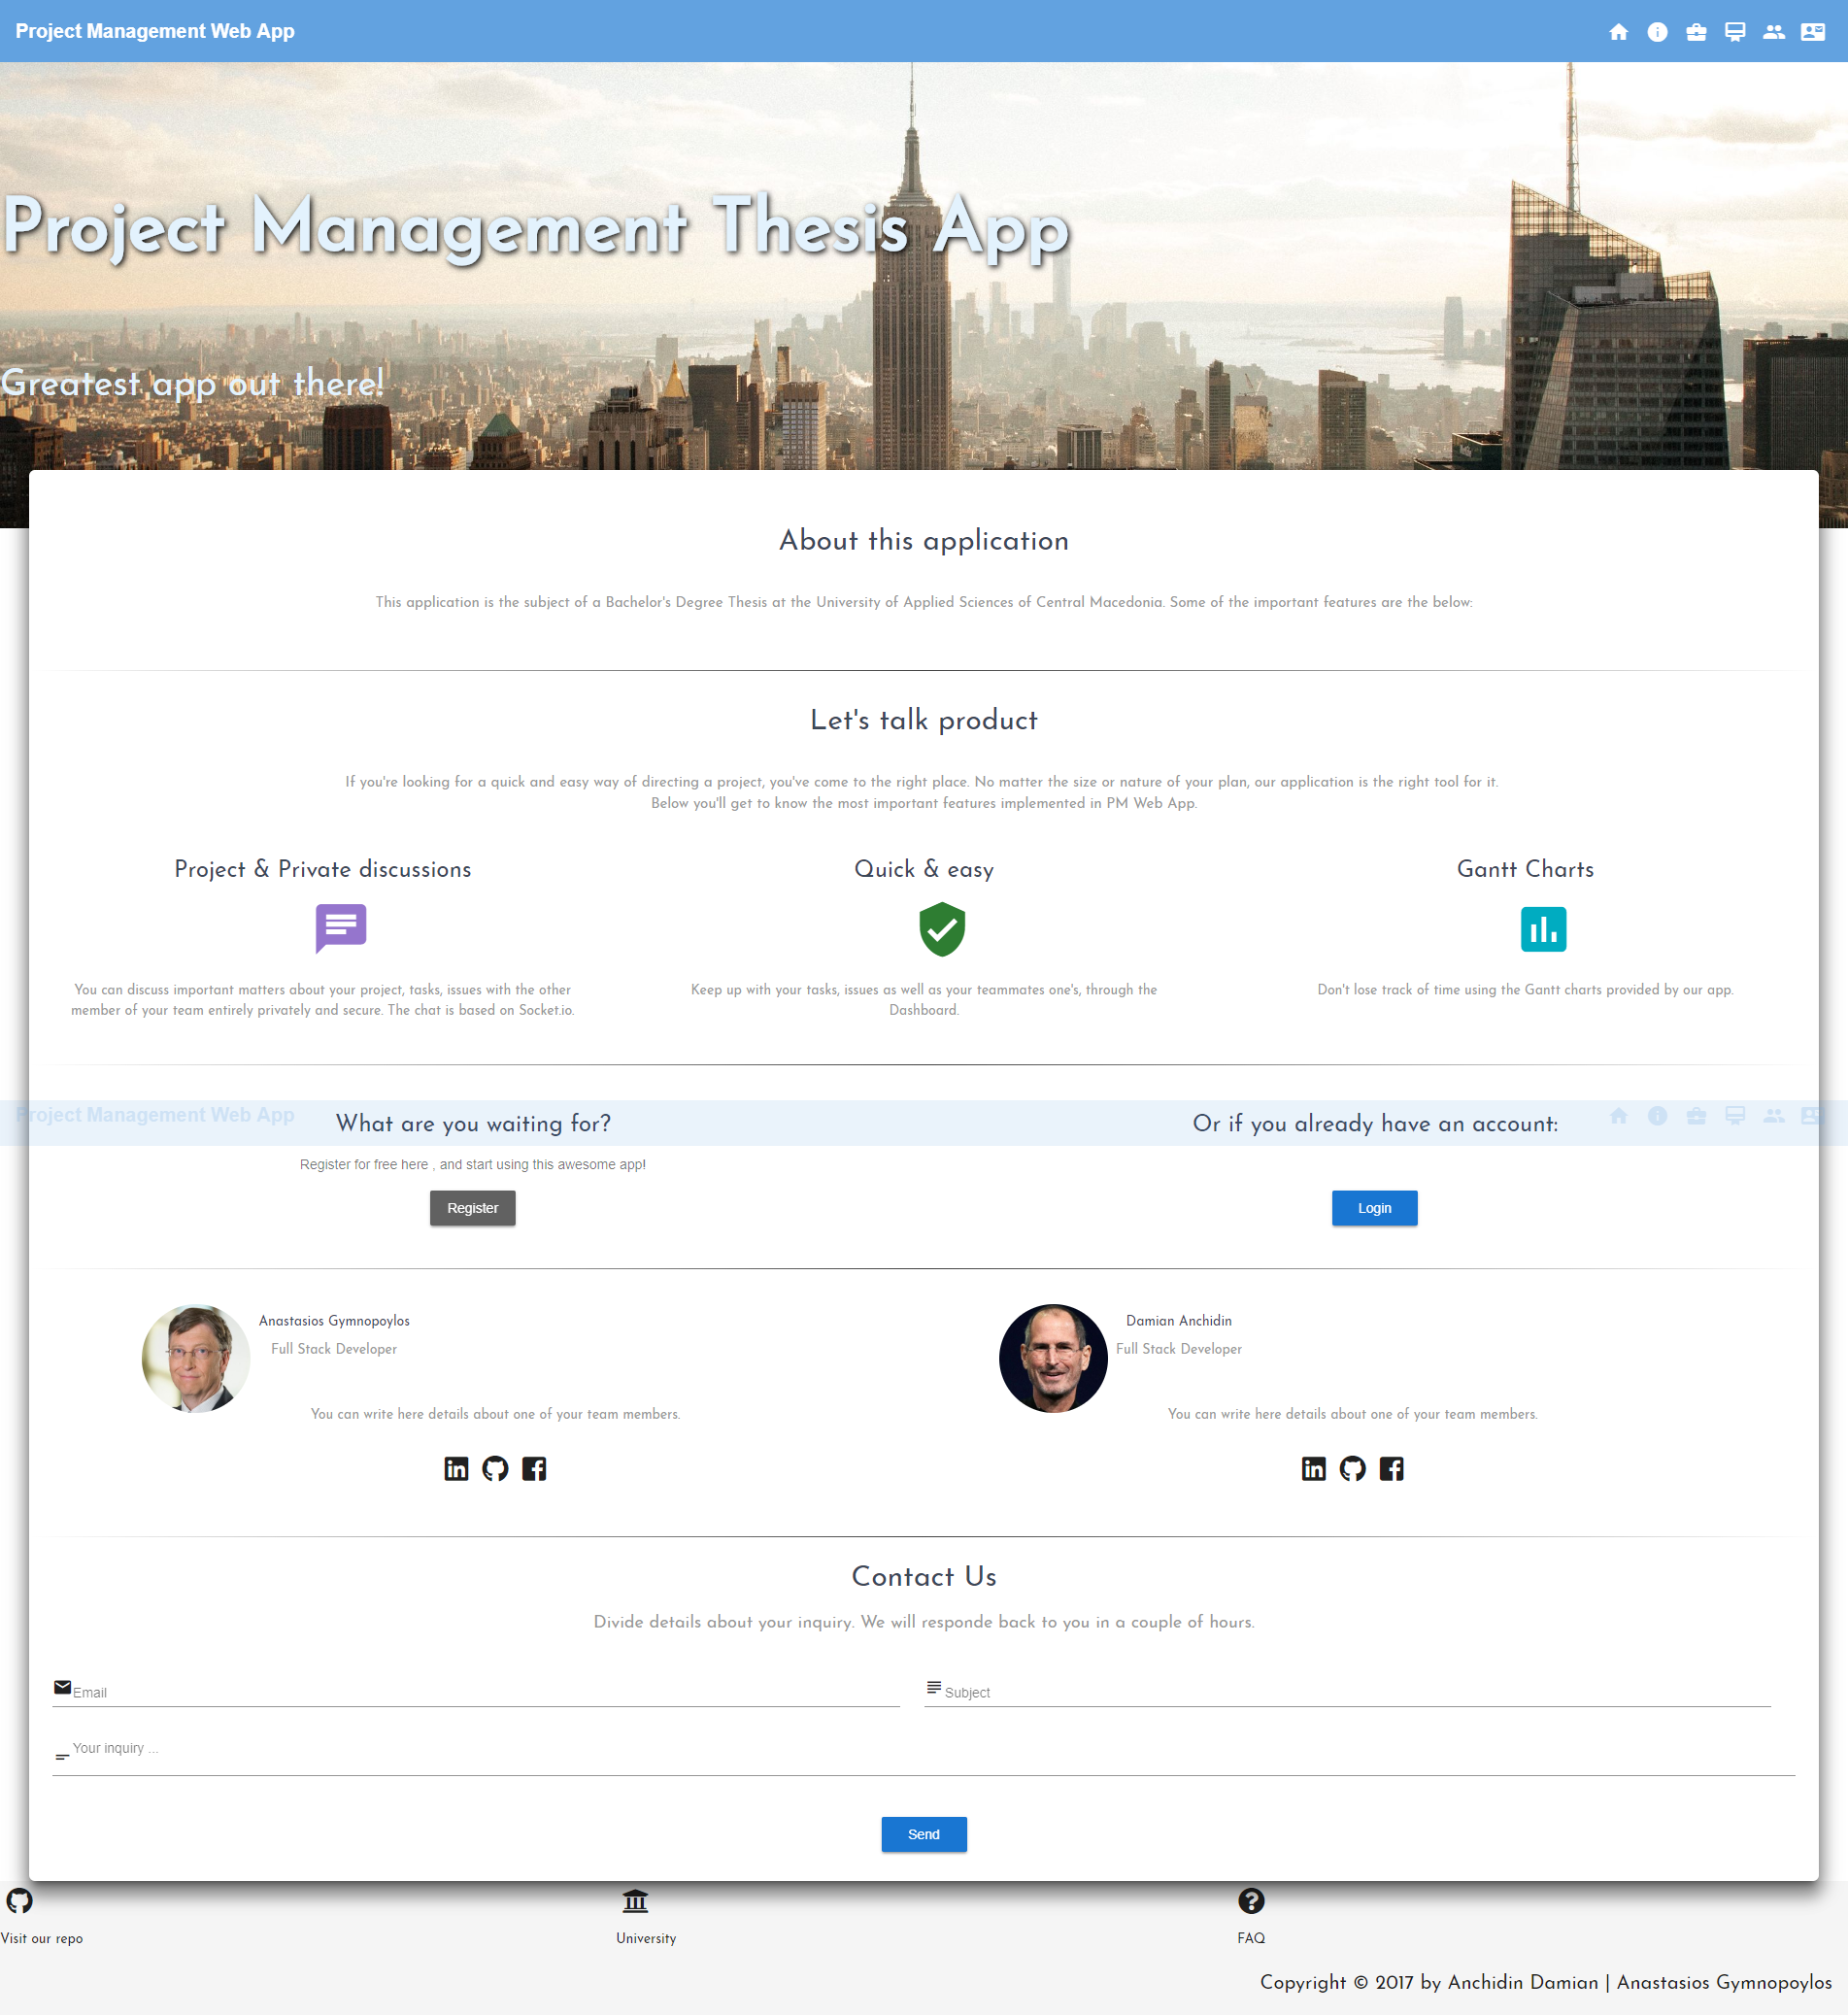
\includegraphics[scale=0.2]{images/homepage.png}
\caption{Αρχική σελίδα - \e{Homepage}}
\label{fig:homepage}
\end{figure}

\section{\e{Authentication}}
\pSpace Ή εφαρμογή απαιτεί ένα λογαριασμό για να αποκτήσει ο χρήστης πρόσβαση στις υπηρεσίες που προσφέρονται. Ή εγγραφή αλλά και η είσοδος ολοκληρώνονται σε πολύ απλά βήματα. Προς το παρόν δεν υπάρχει δυνατότητα εγγραφής/ είσοδο με λογαρισμό κοινωνικού δικτύου. Αν ο χρήστης επιθυμεί να γυρίσει στην αρχική σελίδα, αυτό επιτυγχάνεται χρησιμοποιώντας την επιλογή του μένου που βρίσκεται στο πάνω μέρος της σελίδας. 

\subsection*{\e{Sign Up}}
\pSpace Η εγγραφή του χρήστη ακολουθεί μια βηματική μορφή για μια καλύτερη εμπειρία (βλ. σχ. \ref{fig:register}).\\
\pSpace Τα βήματα πηγαίνουν ως εξής:\\
\begin{itemize}
	\item Αρχικά εμφανίζονται τρία πεδία για την ηλεκτρονική διεύθυνση, κωδικό και επαλήθευση κωδικού .Ο κώδικος πρέπει να έχει μήκος έξι χαρακτήρων και άνω, αλλιώς εμφανίζεται ένα σφάλμα που ενημερώνει τον χρήστη για αυτήν την ιδιότητα. Επίσης υπάρχει δυνατότητα αποκάλυψης κωδικού για διευκόλυνση. Ακόμη, εμφανίζονται σφάλματα σε περίπτωση που οι κωδικοί δεν είναι ίδιοι η αν η διεύθυνση δεν είναι έγκυρη. Για να προχωρήσει στο επόμενο βήμα, δέν πρέπει να υπάρχουν σφάλματα ενεργά.
	\item Δύο ακόμη απαραίτητα πεδία υπάρχουν στο δεύτερο βήμα εγγραφής. Αφορούν το όνομα και το επίθετο του χρήστη.
	\item Στο τελευταίο βήμα, ο χρήστης έχει τρείς επιλογές: να γυρίσει στον προηγούμενο βήμα για να αλλάξει κάποιο πέδιο, \e{reset} φόρμας για να την ξανασυμπληρώσει και ολοκλήρωση διαδικασίας.
\end{itemize}
\pSpace Αφού έχει ολοκληρωθεί με επιτυχία η εγγραφή του χρήστη, θα τον ανακατευθύνει στην σελίδα εισόδου.

\begin{figure}[!htb]
\centering
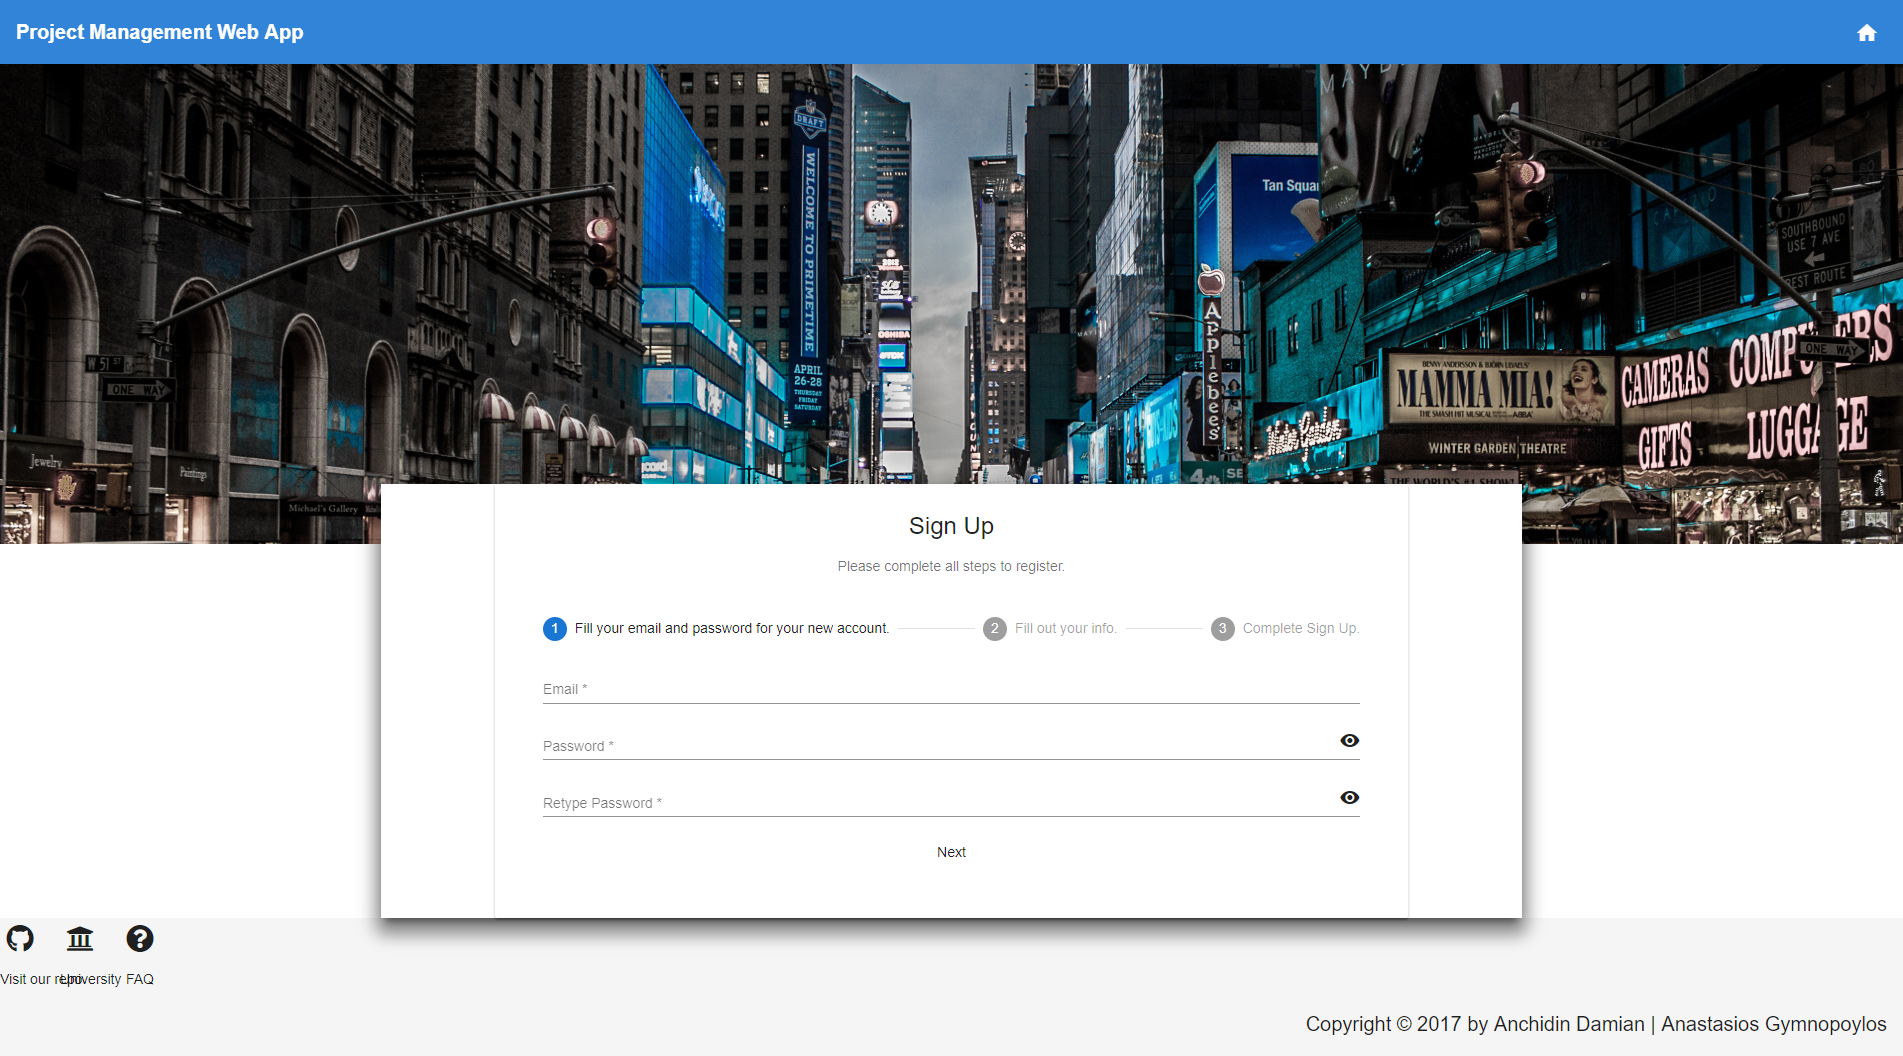
\includegraphics[scale=0.2]{images/register.png}
\caption{Εγγραφή - \e{Sign Up}}
\label{fig:register}
\end{figure}

\subsection*{\e{Sign In}}
\pSpace Συνηθίζεται για την είσοδο σε μια ηλεκτρονική υπηρεσία, να απαιτούνται μια ηλεκτρονική διεύθυνση και ένας κωδικός για επαλήθευση ταυτότητας. Το ίδιο πρότυπο ακολουθείται και στην παρούσα εφαρμογή.\\
\pSpace Ο χρήστης πληκτρολογεί το \e{email} και τον κωδικό, και σε περίπτωση απουσίας κάποιου σφάλματος, θα αποκτήσει πρόσβαση στις υπηρεσίες του \e{iPM}. Τα σφάλματα εμφανίζονται σε ένα \e{modal} παράθυρο με ένα μήνυμα που εξηγεί σε γενικές γραμμές το λάθος. Επίσης, όπως και στην εγγραφή, υπάρχει δυνατότητα αποκάλυψης κωδικού. Αν είναι επιτυχής η είσοδο, θα τον ανακατευθύνει στην εφαρμογή \e{iPM}.

\begin{figure}[!htb]
\centering
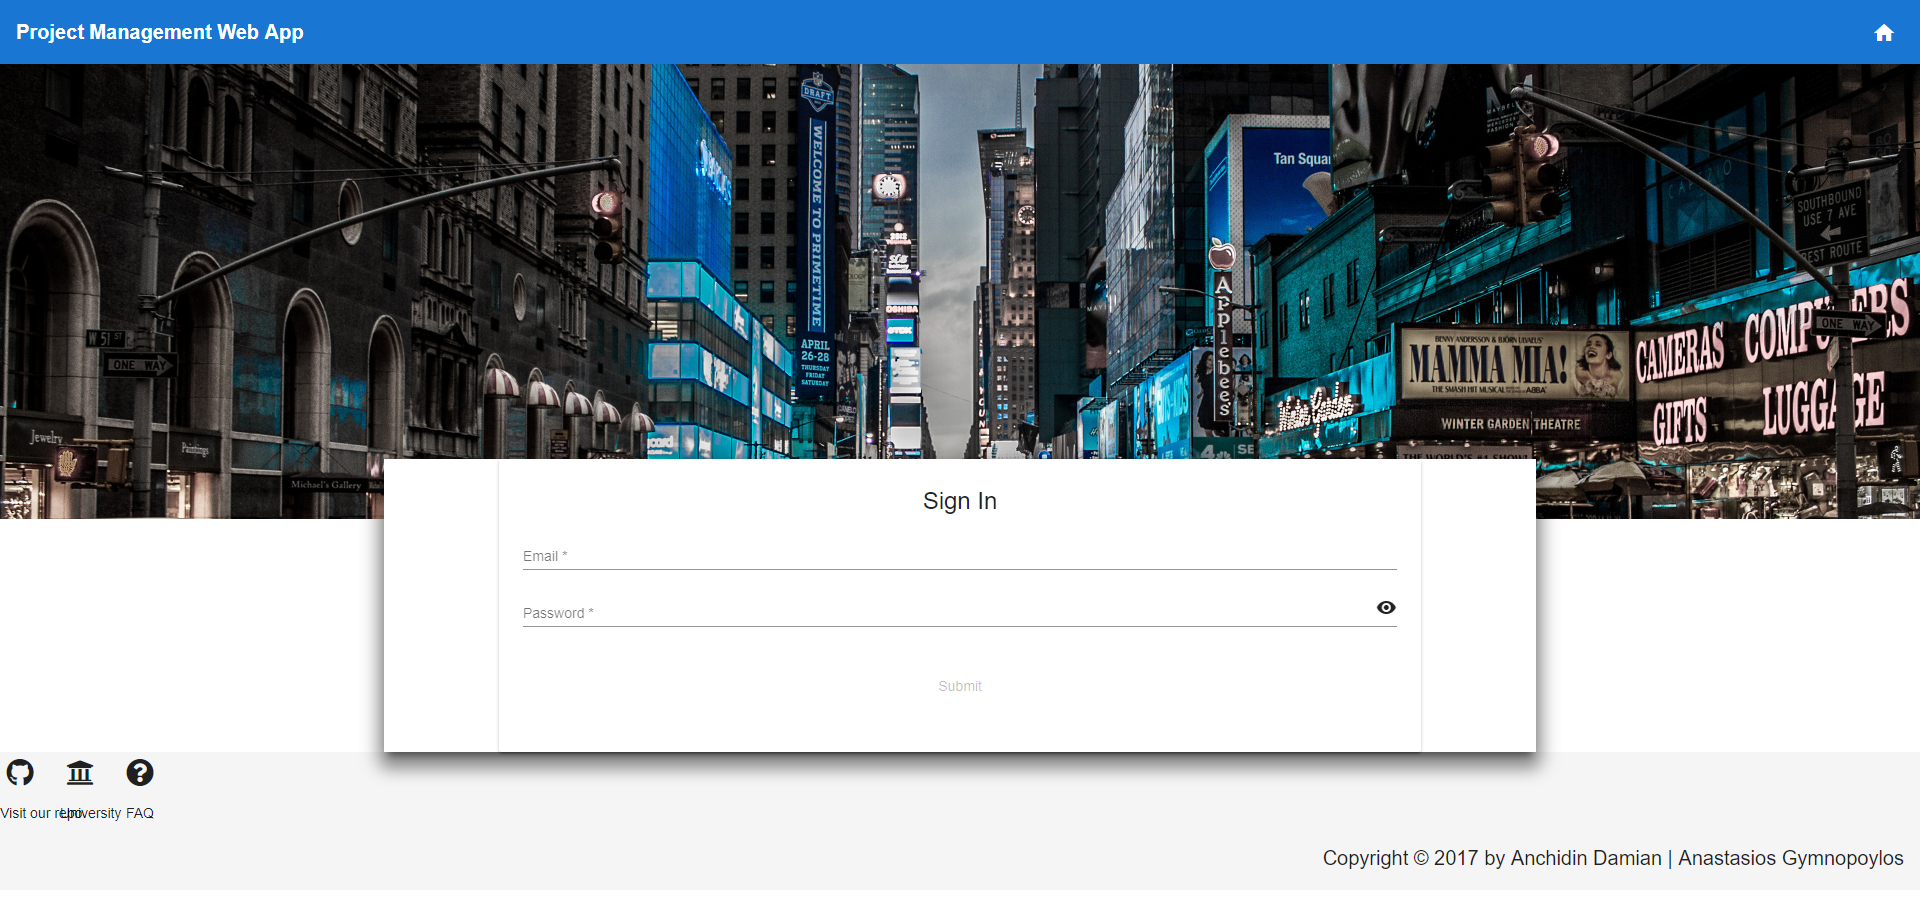
\includegraphics[scale=0.2]{images/login.png}
\caption{Είσοδο - \e{Sign In}}
\label{fig:login}
\end{figure}

\section{\e{iPM}}
\pSpace Εφόσον έχει ολοκληρωθεί το στάδιο ταυτοποιήσης του χρήστη, θα αποκτήσει πρόσβαση στην διεύθυνση \e{\url{https://pmthesis.herokuapp.com/app}} όπου βρίσκεται η εφαρμογή \e{iPM}. Σημειώνεται πώς η εφαρμογή καταλαμβάνει αποθηκευτικό χώρο μέσω του \e{API} του περιηγητή, συγκεκριμένα το \e{Local Storage}. Αποθηκεύονται κάποιες ρυθμίσεις αλλά και το \e{token} που είναι απαραίτητο. Παρ'όλο που το \e{token} μπορεί να τον αποκωδικοποιήσει κανείς και να αλλάξει τις πληροφορίες του, μια τέτοια ενέργεια θα τον ακυρώσει με αποτέλεσμα να ανακατευθύνει τον χρήστη πάλι στην σελίδα εισόδου. Το ίδιο συμβαίνει και στην περίπτωση που λήγει η λείπει το παρόν \e{token}.\\
\pSpace Η σελίδα ακολουθεί τον ίδιο σχεδιασμό και στις δύο περιπτώσεις , χρήστη και έργο. Στο αριστερό μέρος υπάρχει το μενού με τις επιλογές που εξαρτώνται απο την ενότητα που βρίσκεται. Έχει την δυνατότητα απόκρυψης ώστε να μεγαλώσει ο χώρος δεδομένων. Στο επάνω μέρος, υπάρχουν κουμπιά που αφορούν τις ακόλουθες ενέργειες:\\
\begin{itemize}
	\item Το πρώτο στην σειρά είναι ένας διακόπτης για την απόκρυψη του αριστερού μενού.
	\item Δεύτερο είναι μια συντόμευση που επαναφέρει τον χρήστη στην αρχική σελίδα του \e{iPM}.
	\item Στην συνέχεια φαίνεται ένα πεδίο \e{Search} όπου ο χρήστης μπορεί να ψάξει έργα, άτομα και \e{task} για να διευκολυνθεί η διαχείριση έργων και εργασιών.
	\item Το επόμενο κουμπί εμφανίζει στο δεξί μέρος της σελίδας τις ειδοποιήσεις.
	\item Ακολουθεί ένα κουμπί το όποιο ανοιγεί ένα μικρό \e{Context Menu} που περιέχει τέσσερις επιλογές για το θέμα σχεδιασμού.
	\item Τελευταίο είναι η αποσύνδεση, που ανακατευθύνει τον χρήστη στην σελίδα σύνδεσης.
\end{itemize}
\pSpace Στον υπόλοιπο χώρο φορτώνεται το δυναμικό περιεχόμενο. Θα αναφέρεται παρακάτω ως πλαίσιο δεδομένων.

% User actions
\subsection{\e{User}}
\pSpace Αρχικά η εφαρμογή καλωσορίζει τον χρήστη, με τις ενέργειες που αφορούν τον ίδιο. Το μενού περιλαμβάνει τις ακόλουθες επιλογές, οι οποίες εξηγούνται σε λεπτομέρεια παρακάτω:\\
\begin{itemize}
	\item \e{Dashboard}
	\item \e{My Projects}
	\item \e{My Tasks}
	\item \e{My Issues}
	\item \e{My Profile}
	\item \e{Calendar}
	\item \e{Chat}
	\item \e{Invites}
	\item \e{404}
\end{itemize} 

\subsubsection*{\e{Dashboard}}
\pSpace Το \e{Dashboard} (βλ. σχ. \ref{fig:userDashboard}) βρίσκεται στην διεύθυνση \e{\url{http://pmthesis.herokuapp.com/app/dashboard}} και φορτώνει στον πλαίσιο δεδομένων, πέντε καρτέλες:
\begin{itemize}
	\item Η πρώτη είναι μια δοκιμστική καρτέλα, στην οποία ο χρήστης αλλάζει το μέγεθος καρτέλων.
	\item Η δεύτερη εμφανίζει τα \e{Tasks} που είναι ανατεθημένα στον ίδιο, στα οποία έχει περάσει ο χρόνος ολοκλήρωσης. Προς το παρόν δείχνει μόνο απλά \e{Tasks}.
	\item Η επόμενη καρτέλα προσφέρει συντομεύσεις για τα ενεργά έργα.
	\item Στην τέταρτη καρτέλα, περιέχονται τα πιο πρόσφατα \e{Tasks} που ανατέθηκαν στον χρήστη.
	\item Η τελευταία καρτέλα έχει την ίδια λειτουργία με την προηγούμενη, αλλά για τα \e{Issues}.
\end{itemize}

\pSpace Στις καρτέλες που περιέχουν τα \e{tasks, issues}, επιλέγοντας κάποιο απο αυτά, ανακατευθύνει τον χρήστη στην διεύθυνση \e{\url{https://pmthesis.herokuapp.com/app/assignmentview/@id}}. Επίσης η επιλογή ενός έργου απο την τρίτη καρτέλα, ανοίγει την ενότητα έργου με τις πληροφορίες του.

\begin{figure}[!htb]
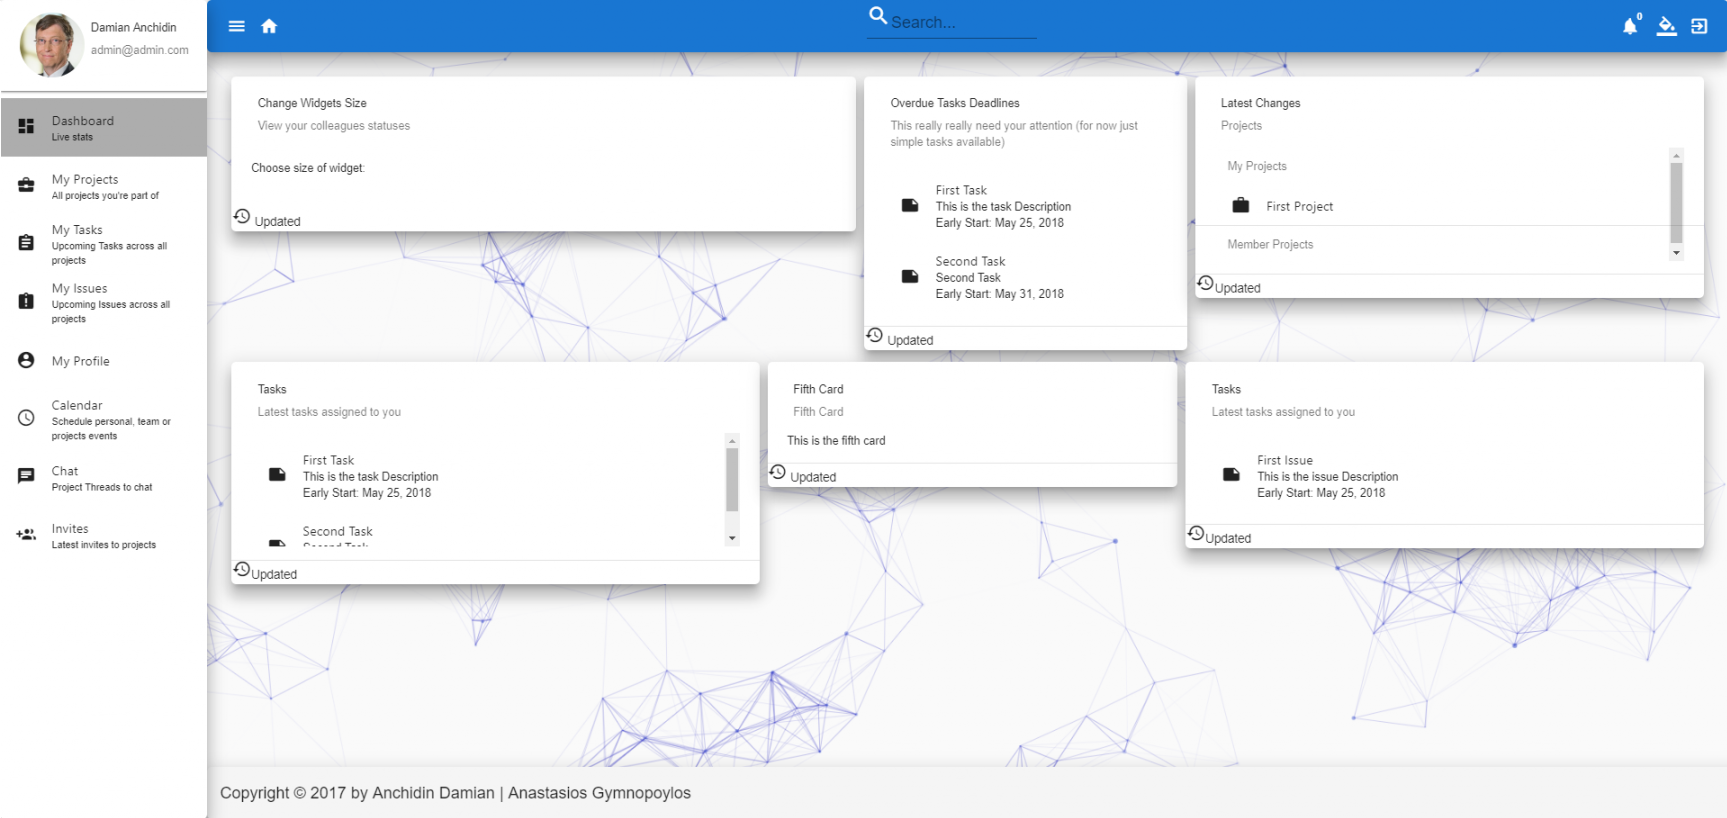
\includegraphics[width=\columnwidth, height=10cm]{images/userDashboard.png}
\caption{\e{User - Dashboard}}
\label{fig:userDashboard}
\end{figure}

\subsubsection*{\e{My Projects}}
\pSpace Η επιλογή \e{My Projects} από το αριστερό μενού της \e{iPM} φορτώνει στον πλαίσιο δεδομένων μια καρτέλα με τα ενεργά έργα του χρήστη (διαχειριστής η μέλος), αλλά και την δυνατότητα δημιουργίας νέου έργου. Η νέα διεύθυνση πλέον είναι \e{\url{https://pmthesis.herokuapp.com/app/myprojects}} (βλ. σχ. \ref{fig:userMyProjects}).

\begin{figure}[!htb]
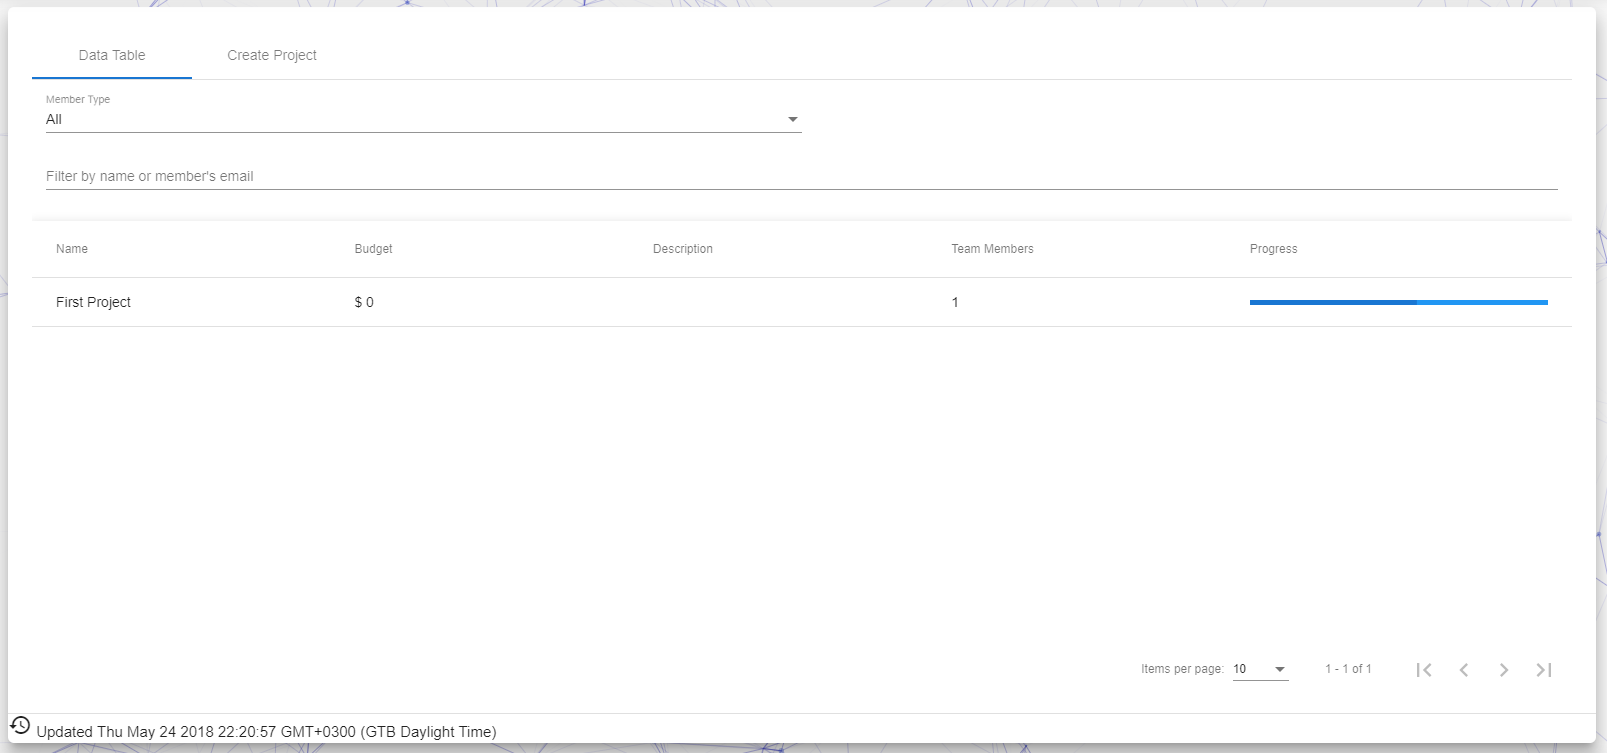
\includegraphics[width=\columnwidth, scale=4]{images/userMyProjects.png}
\caption{\e{User - My Projects}}
\label{fig:userMyProjects}
\end{figure}

\pSpace Στο πρώτο \e{tab} φαίνεται ο πίνακας με τα έργα του χρήστη. (σχ. \ref{fig:userMyProjects}). Κάθε εγγραφή αποτελείται από πέντε ιδιότητες: όνομα, προϋπολογισμός, μια σύντομη περιγραφή (εμφανίζονται μόνο 60 χαρακτήρες), μέγεθος ομάδας και η πρόοδος απεικονιζόμενη σε γραμμή προόδου.  Επιλέγοντας κάποιο έργο, ανοίγει την "σελίδα" του έργου.\\
\pSpace Ο πίνακα διαθέτει σελιδοποίηση και ρύθμιση για τον σύνολο εγγραφών ανά σελίδα. Επιπλέον, πάνω από τον πίνακα υπάρχουν δύο πεδία που επιτρέπουν αλληλεπίδραση με τον χρήστη.\\
\pSpace Το πρώτο είναι τύπου \e{Select} και περιέχει τρείς επιλογές: \e{all, manager, member}, με την πρώτη να είναι η προκαθορισμένη. Σύμφωνα με την επιλεγμένη τιμή, ο πίνακας φιλτράρεται, εμφανίζοντας όλα τα έργα, έργα στα οποία ο χρήστης είναι διαχειριστής, ή έργα στα οποία είναι μέλος.\\
\pSpace Στο δεύτερο πεδίο, ο χρήστης πληκτρολογεί ένα όνομα η μια ηλεκτρονική διεύθυνση και ο πίνακας φιλτράρεται με βάση αυτών. Σημειώνεται πώς τα δύο πεδία λειτουργούν ταυτοχρόνος, δηλαδή το αποτέλεσμα επηρεάζεται και απο τις δύο επιλογές.\\

\pSpace Συνεχίζοντας στον δεύτερο \e{tab}, \e{Create Project} (βλ. σχ. \ref{fig:userCreateProject1}), δίνεται η δυνατότητα δημιουργίας νέου έργου. Η λειτουργία αυτή ακολουθεί βηματική μορφή αποτελούμενο από τρία στάδια.\\
\pSpace Στο πρώτο βήμα, εισάγονται οι βασικές πληροφορίες του έργου, δηλαδή:\\
\begin{itemize}
	\item Η εταιρία που διαχειρίζει το εν λόγω έργο
	\item Τύπο έργο, ιδιωτικό η δημόσιο
	\item Όνομα έργου
	\item Προυπολογισμός
	\item Σύντομη περιγραφή
\end{itemize}

\begin{figure}[!htb]
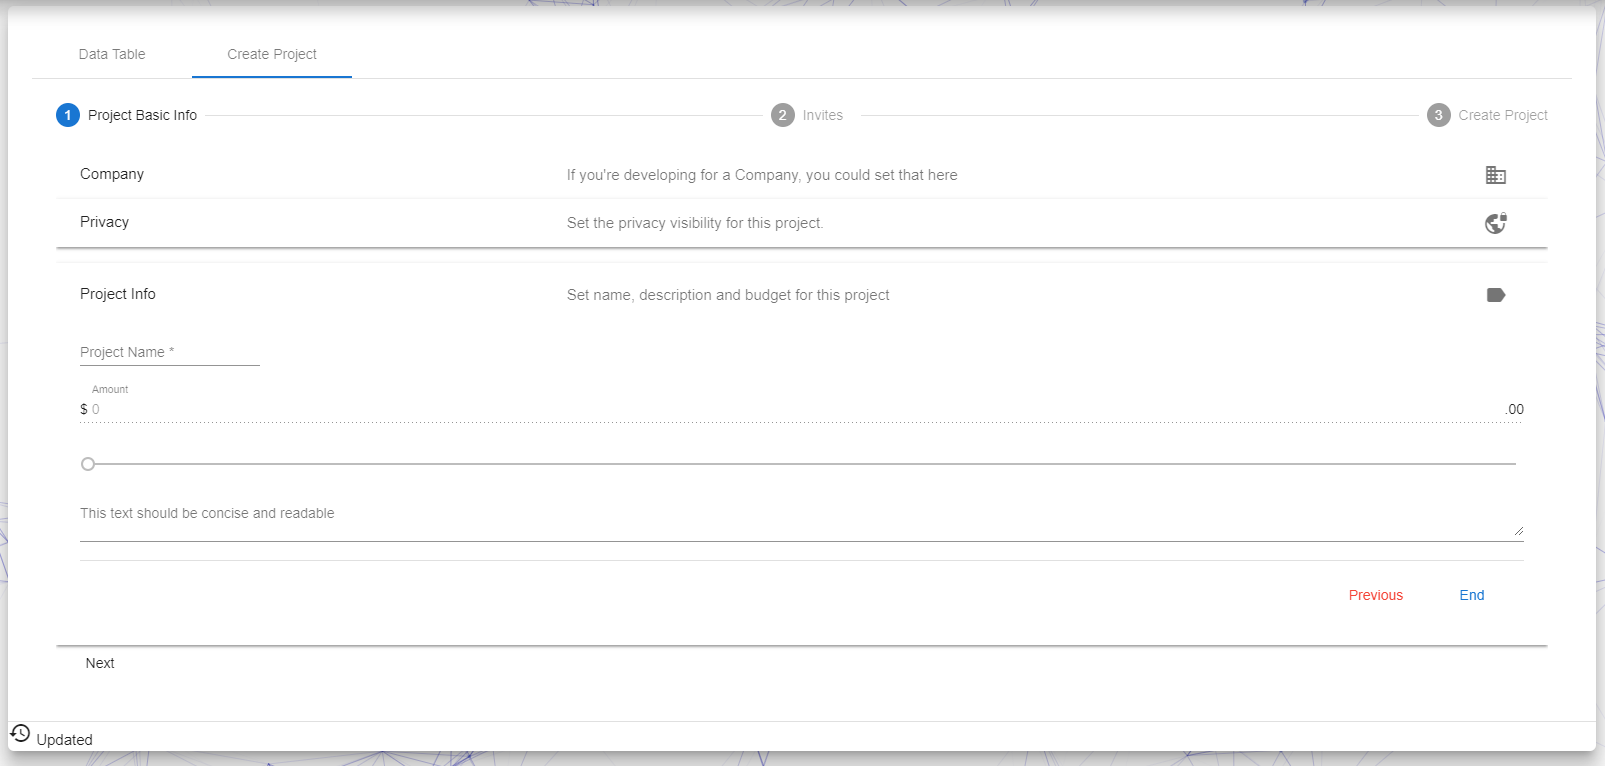
\includegraphics[width=\columnwidth, scale=4]{images/userCreateProject1.png}
\caption{\e{User - Create Project}}
\label{fig:userCreateProject1}
\end{figure}

\pSpace Ο τύπος έργου, επιλέγεται με την βοήθεια ενός \e{Slide-Toggle}, και ο προυπολογισμός με έναν ολισθητή (\e{slider}) το οποίο έχει μέγιστη τιμή 50.000 .Τα υπόλοιπα είναι τα συνηθισμένα πεδία για εισαγωγή κειμένου. Για να περάσει στον επόμενο βήμα, είναι απαραίτητο να συμπληρωθεί το όνομα έργου.\\

\pSpace Στο δεύτερο βήμα (βλ. σχ. \ref{fig:userCreateProject2}), ο χρήστης μπορεί να καλέσει άτομα να συμβάλλουν στην ανάπτυξη έργου. Καθώς πληκτρολογεί μια ηλεκτρονική διεύθυνση στο πεδίο, εμφανίζονται απο κάτω \e{emails} υπαρκτών λογαριασμών. Επιλέγοντας κάποιο, τον προσθέτει στην λίστα προσκλήσεων. Επιπλέον, αν ο χρήστης πληκτρολογεί το κόμμα, προσθέτει αυτομάτως την διεύθυνση. Έτσι, αν οι διευθύνσεις είναι σωστές, η διαδικασία αυτή επιτυγχάνεται πιο γρήγορα. Ακόμη, αν ο χρήστης προσπαθεί να προσθέσει τον ίδιο, η λογαριασμό που δεν υπάρχει, εμφανίζεται ένα σφάλμα με μια σύντομη περιγραφή.

\begin{figure}[!htb]
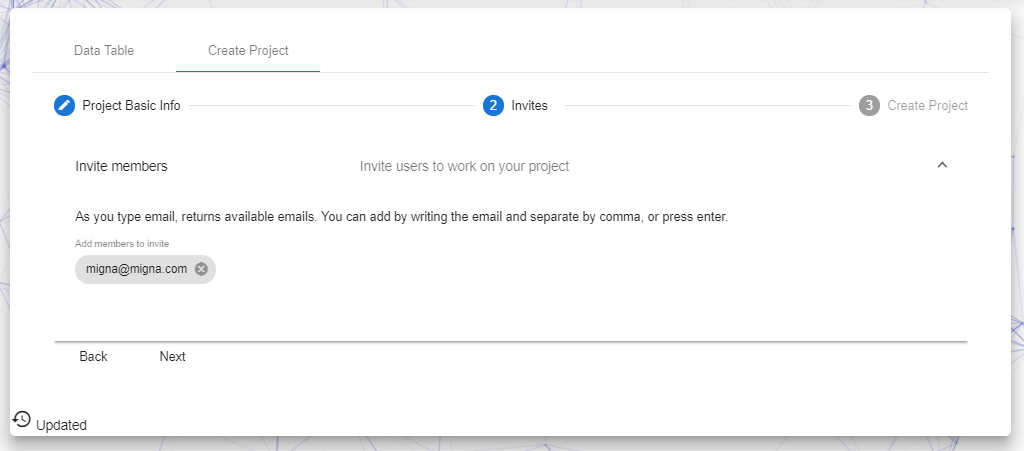
\includegraphics[width=\columnwidth, scale=4]{images/userCreateProject2.png}
\caption{\e{User - Create Project}}
\label{fig:userCreateProject2}
\end{figure}

\pSpace Το τελευταίο βήμα, εμφανίζει τις πληροφορίες του έργου που θα δημιουργηθεί αλλά και τρείς επιλογές: γύρισμα στο προηγούμενο βήμα, \e{reset} και ολοκλήρωση διαδικασίας. Αν ληφθεί επιτυχής μήνυμα, αλλάζει το \e{tab} στο αρχικό που εμφανίζονται τα έργα, όπου πλέον παρατηρείται και το καινούργιο.

\subsubsection*{\e{My Tasks}}
\pSpace Ο χρήστης παρακολουθεί τα \e{Tasks} που του έχουν ανατεθεί, επιλέγοντας \e{My Tasks} από το αριστερό μενού η πηγαίνοντας στην διεύθυνση \e{\url{https://pmthesis.herokuapp.com/app/mytasks}}. Στο πλαίσιο δεδομένων, εμφανίζεται μια καρτέλα με ένα διάγραμμα (βλ. σχ. \ref{fig:userTasks}) που θυμίζει \e{Gantt}.\\
\pSpace Το εν λόγω διάγραμμα, περιέχει όλα τα \e{Tasks} που δεν έχουν ολοκληρωθεί, ανά έργο, σημειώντας και το διάστημα χρόνου τους. Για καλύτερη εμπειρία χρήσης, ένα έργο μπορεί να συρρικνωθεί σε περίπτωση που ο χρήστης θέλει να το αγνοήσει.\\
\pSpace Επιπλέον, το διάγραμμα προσφέρει την δυνατότητα εκτύπωσής της, η κατεβάσματος. Στην αριστερή γωνία, επιλέγοντας το κουμπί, ανοίγει ένα \e{Context Menu} με τέσσερις επιλογές: εκύπωση και κατέβασμα υπο διαφορετικές μορφές (\e{PNG, JPG, PDF, SVG}).

\begin{figure}[!htb]
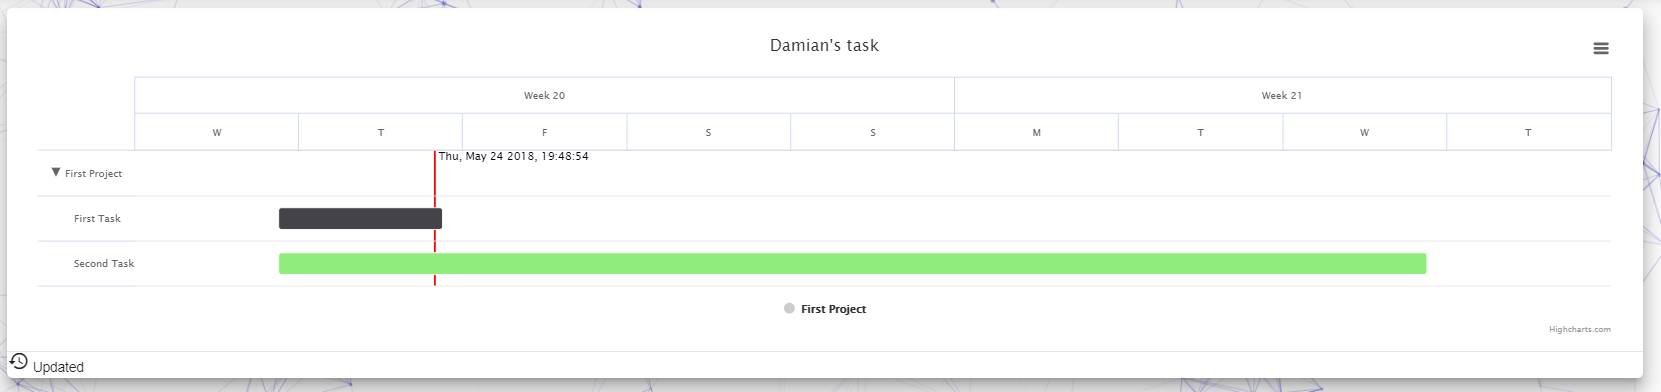
\includegraphics[width=\columnwidth, height=8cm]{images/userTasks.png}
\caption{\e{User - Tasks}}
\label{fig:userTasks}
\end{figure}

\subsubsection*{\e{My Issues}}
\pSpace Προχωρόντας στο \e{My Issues}, παρατηρείται ότι η καρτέλα (βλ. σχ. \ref{fig:userIssues}) που φορτώνεται στο πλαίσιο δεδομένων στην διεύθυνση \e{\url{https://pmthesis.herokuapp.com/app/myissues}}, είναι ίδια με την προηγούμενη (βλ. σχ. \ref{fig:userTasks}). Διαφέρουν στα δεδομένα που εμφανίζονται, καθώς εδώ υπάρχουν μόνο τα \e{Issues}, oι λειτουργίες όμως παραμένουν ίδιες.

\begin{figure}[!htb]
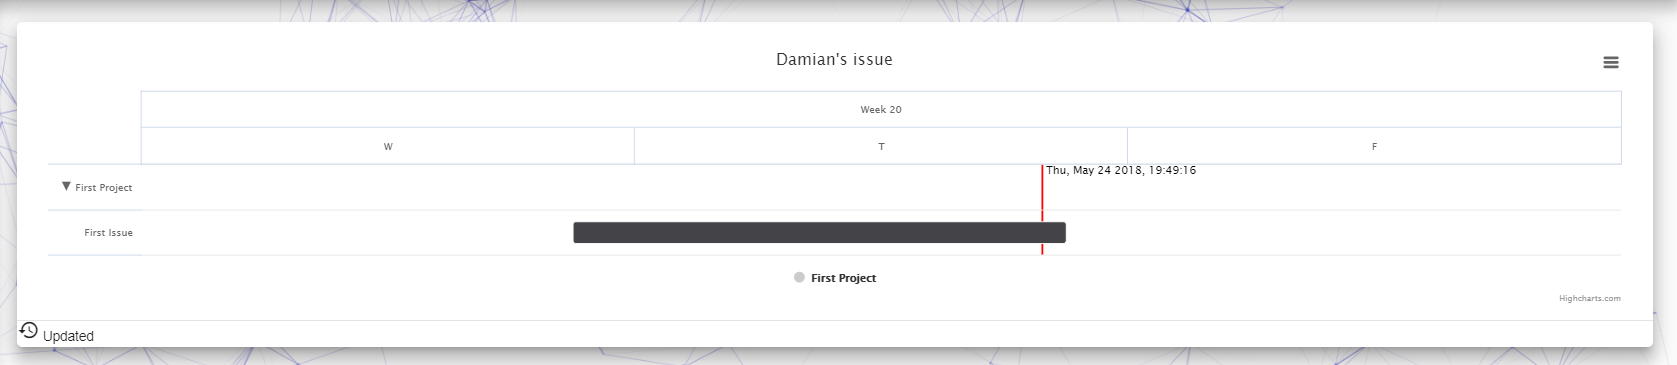
\includegraphics[width=\columnwidth, height=8cm]{images/userIssues.png}
\caption{\e{User - Issues}}
\label{fig:userIssues}
\end{figure}

\subsubsection*{\e{My Profile}}
\pSpace Η πέμπτη επιλογή του αριστερού μενού, \e{My Profile}, αλλάζει την διεύθυνση σε \e{\url{https://pmthesis.herokuapp.com/app/profile}} και φορτώνει στο πλαίσιο δεδομένων μια καρτέλα η οποία περιέχει τις πληροφορίες του χρήστη (βλ. σχ. \ref{fig:userProfile}).\\
\pSpace Για να πετύχει μια καλύτερη διοργάνωση των πληροφοριών και μια γρήγορη διαχείρισή τους ως αποτέλεσμα, προσθέτηκαν \e{Expansion Panels}, τα όποια κατέχουν ένα όνομα και μια σύντομη περιγραφή έτσι ώστε ο χρήστης να ανοίξει μόνο αυτό που επιθυμεί να αλλάξει η να δεί χωρίς να μετακινείται προς τα κάτω συνέχεια.\\
\pSpace Υπάρχουν πέντε \e{Expansion Panels}:\\

\begin{figure}[!htb]
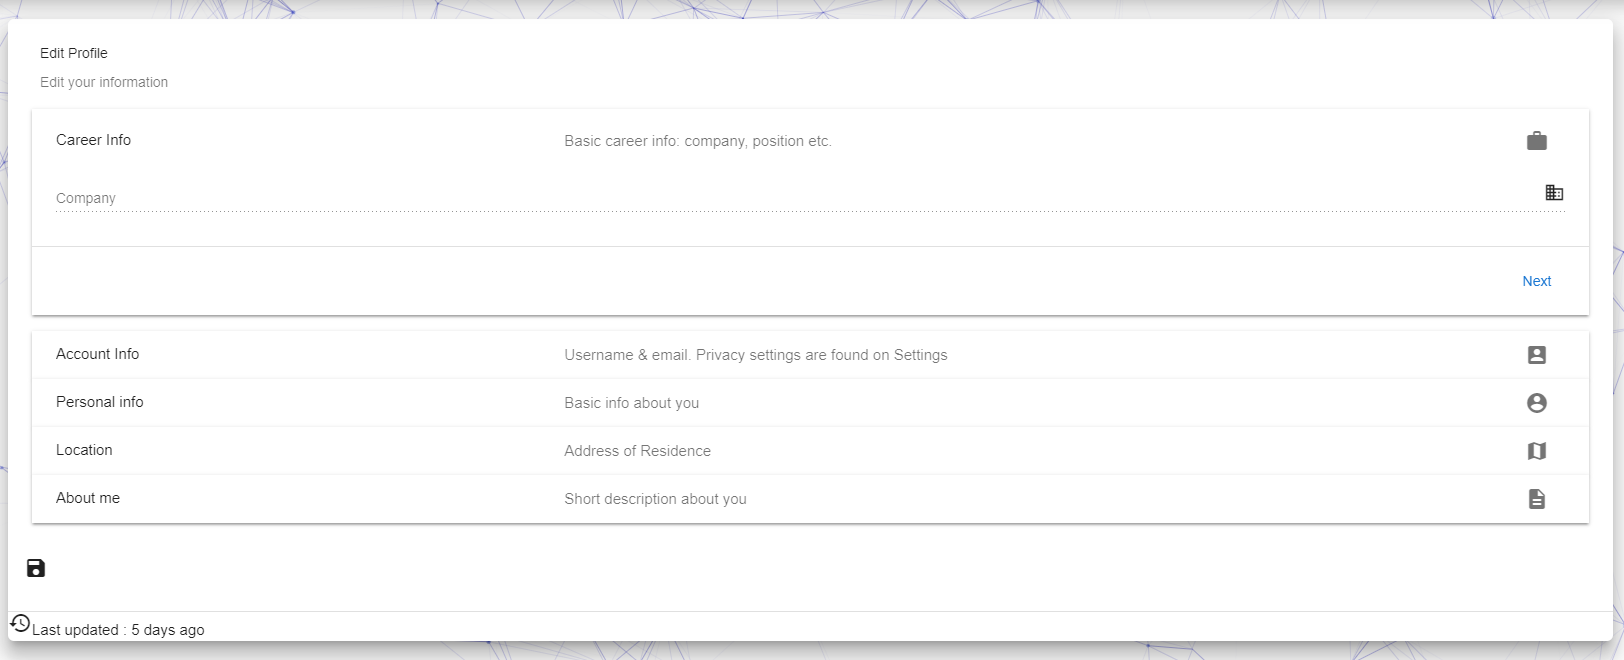
\includegraphics[width=\columnwidth, height=8cm]{images/userProfile.png}
\caption{\e{User - Profile}}
\label{fig:userProfile}
\end{figure}

\begin{itemize}
	\item \e{Career Info} - Προς το παρόν περιλαμβάνει ένα πεδίο όπου πληκτρολογείται η εταιρία στην όποια δουλεύει ο χρήστης.
	\item \e{Account Info} - Πληροφορίες που αφορούν τον λογαριασμό. Δύο πεδία κειμένου αποτελούν τον \e{panel} αυτό, ένα που αφορά την ηλεκτρονική διεύθυνση που δεν αλλάζει, και ένα για το \e{username} που επιθυμεί ο χρήστης να τον αντιπροσωπεύει.
	\item \e{Personal Info} - Δύο πεδία κειμένου επίσης και έδω, για το όνομα και το επίθετο του χρήστη.
	\item \e{Location} - Περιλαμβάνει τρία πεδία κειμένου για την διεύθυνση, πόλη, ταχυδρομικός κώδικας (μόνο αριθμητικύς χαρακτήρες) και ένα πεδίο τύπου \e{Select} όπου ο χρήστης μπορεί να επιλέξει την χώρα. Το τελευταίο πεδίο έχει την δυνατότητα αυτόματης συμπλήρωσης, δηλαδή καθώς πληκτρολογείται η ονομασία μιας χώρας, εμφανίζονται απο κάτω πιθανά αποτελέσματα μαζί με την σημαία (βλ. σχ. \ref{fig:userProfileCountry}).
	\item \e{About me} - Εδώ ο χρήστης μπορεί να περιγράψει τον εαυτό του σε ένα κείμενο μέγιστο μέγεθος 255 χαρακτήρων. Καθώς γράφει, στην δεξιά γωνία του πεδίου κειμένου, εμφανίζεται το τρέχων σύνολο χαρακτήρων.
\end{itemize}

\begin{figure}[!htb]
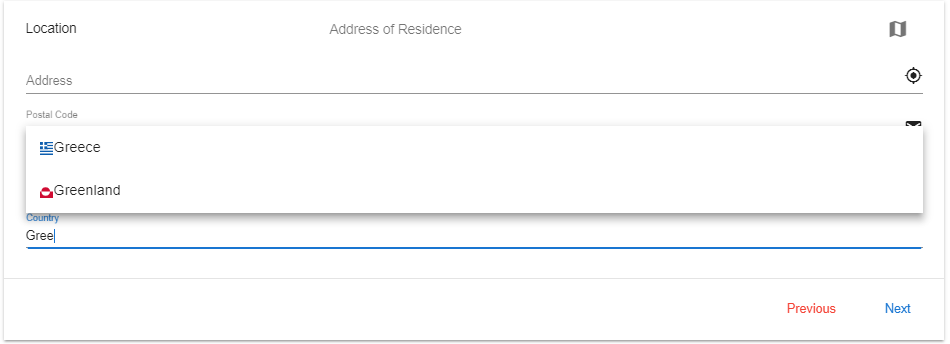
\includegraphics[width=\columnwidth, scale=4]{images/userProfileCountry.png}
\caption{\e{User - Select Country}}
\label{fig:userProfileCountry}
\end{figure}

\pSpace Αν αποφασίσει να αλλάξει κάποιες από αυτές τις πληροφορίες ο χρήστης και επιθυμεί να τα αποθηκεύσει, αυτό επιτυγχάνεται με το κουμπί που βρίσκεται στην αριστερή γωνία της καρτέλας.\\
\pSpace Επιπλέον, υπάρχει και μια ακόμη διεύθυνση που αφορά το προφίλ ενός χρήστη \e{\url{https://pmthesis.herokuapp.com/app/profile/@email}}. Αντί για το \e{@email} ο χρήστης πληκτρολογεί την ηλεκτρονική διεύθυνση ενός υπαρκτού λογαριασμού. Οι πληροφορίες που εμφανίζονται είναι ελάχιστες προς το παρών. Ακόμη, αν πληκτρολογεί την δική του διεύθυνση, ανακατευθύνεται στην απλή διεύθυνση που αναφέραμε πιο πάνω.

\subsubsection*{\e{Calendar}}
\pSpace Το ημερολόγιο είναι ένα απο τα πιο απαραίτητα εργαλεία στο \e{Project Management}. Η διεύθυνση \e{\url{https://pmthesis.herokuapp.com/app/calendar}} φορτώνει στο πλαίσιο δεδομένων μια καρτέλα που περιέχει ένα ημερολόγιο (βλ. σχ. \ref{fig:userCalendar}).\\
\pSpace Παρατηρείται πως στο πάνω μέρος της καρτέλας ύπάρχει μια ομάδα κουμπιών (\e{Month, Week, Day}), στην οποία μόνο ένα μπορεί να είναι επιλεγμένο ανα δεδομένη στιγμή. Απο κάτω, τρία κουμπιά (\e{Previous, Today, Next}) προσφέρουν την δυνατότητα περιήγησης (εξηγείται παρακάτω).\\
\pSpace Επιλέγοντας το \e{Month} η καρτέλα εμφανίζει τον τρέχων μήνα (βλ. σχ. \ref{fig:userCalendar}). Στις ημέρες που υπάρχουν σύμβαντα, το κελί της ημέρας δείχνει τον σύνολό τους, και αν επιλεχτεί η ημέρα, εμφανίζεται μια λίστα με τα σύμβαντα ανά κατηγορία. Τα τρία κουμπιά περιήγησης, σε αυτήν την περίπτωση δείχνουν τον προηγούμενο μήνα, τρέχων και επόμενο μήνα.

\begin{figure}[!htb]
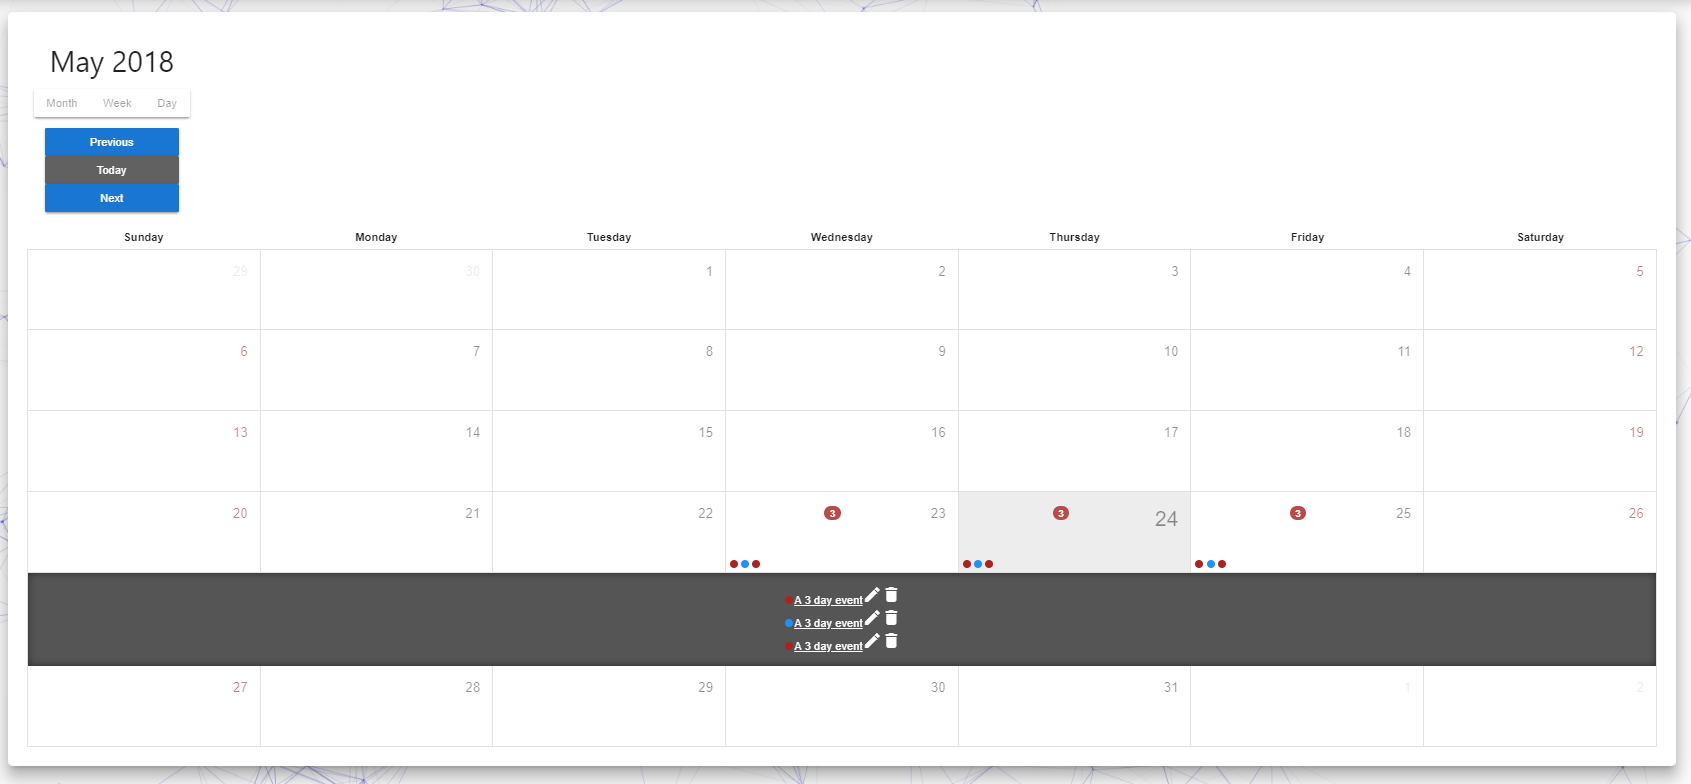
\includegraphics[width=\columnwidth, height=8cm]{images/userCalendar.png}
\caption{\e{User - Calendar Month}}
\label{fig:userCalendar}
\end{figure}

\pagebreak

\pSpace Η δεύτερη επιλογή της ομάδας κουμπιών, εμφανίζει την τρέχων εβδομάδα (βλ. σχ. \ref{fig:userCalendarWeek}). Τα κουμπιά περιήγησης, δείχνουν την προηγούμενη εβδομάδα, τρέχων και επόμενη.

\begin{figure}[!htb]
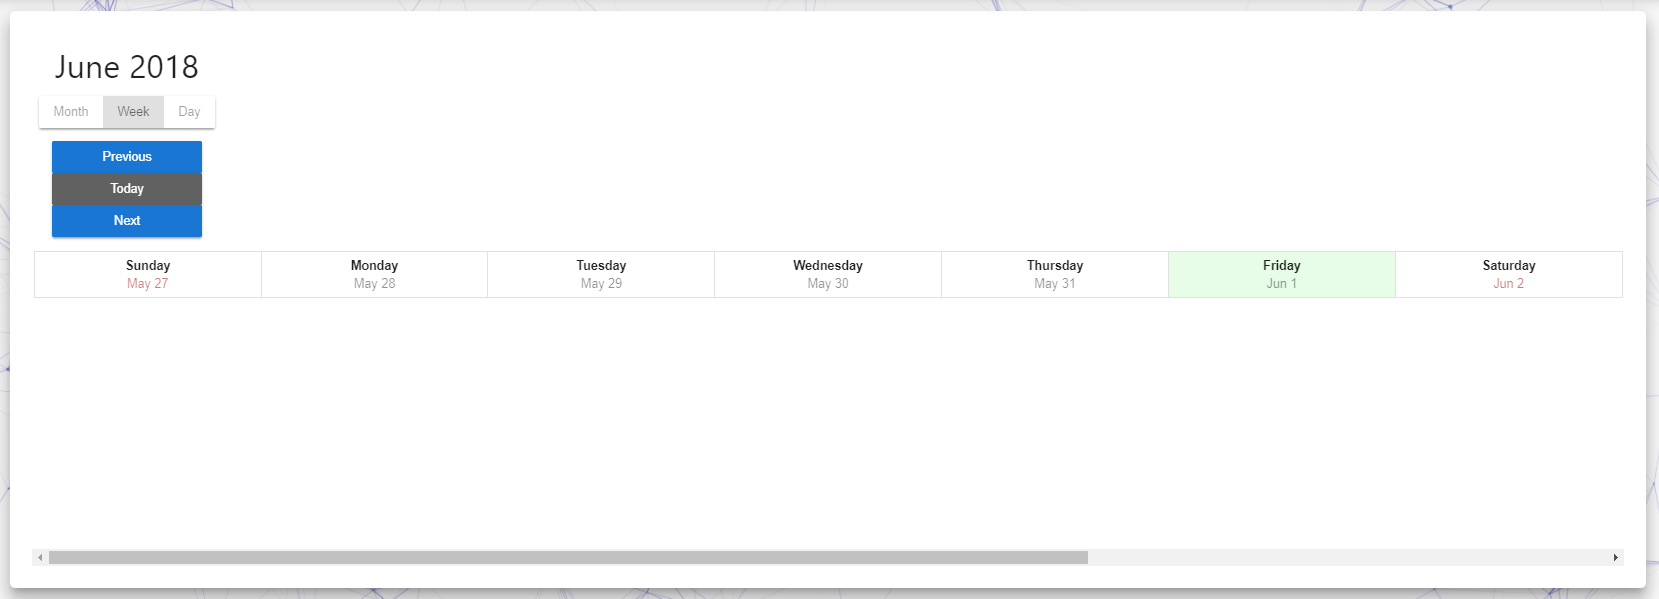
\includegraphics[width=\columnwidth, height=8cm]{images/userCalendarWeek.png}
\caption{\e{User - Calendar Week}}
\label{fig:userCalendarWeek}
\end{figure}

\pSpace Η τελευταία επιλογή, \e{Day}, εμφανίζει την τρέχων ημέρα (βλ. σχ. \ref{fig:userCalendarDay}) και τα κουμπιά περιήγησης δείχνουν την προηγούμενη μέρα, σημερινή και την επομένη.

\begin{figure}[!htb]
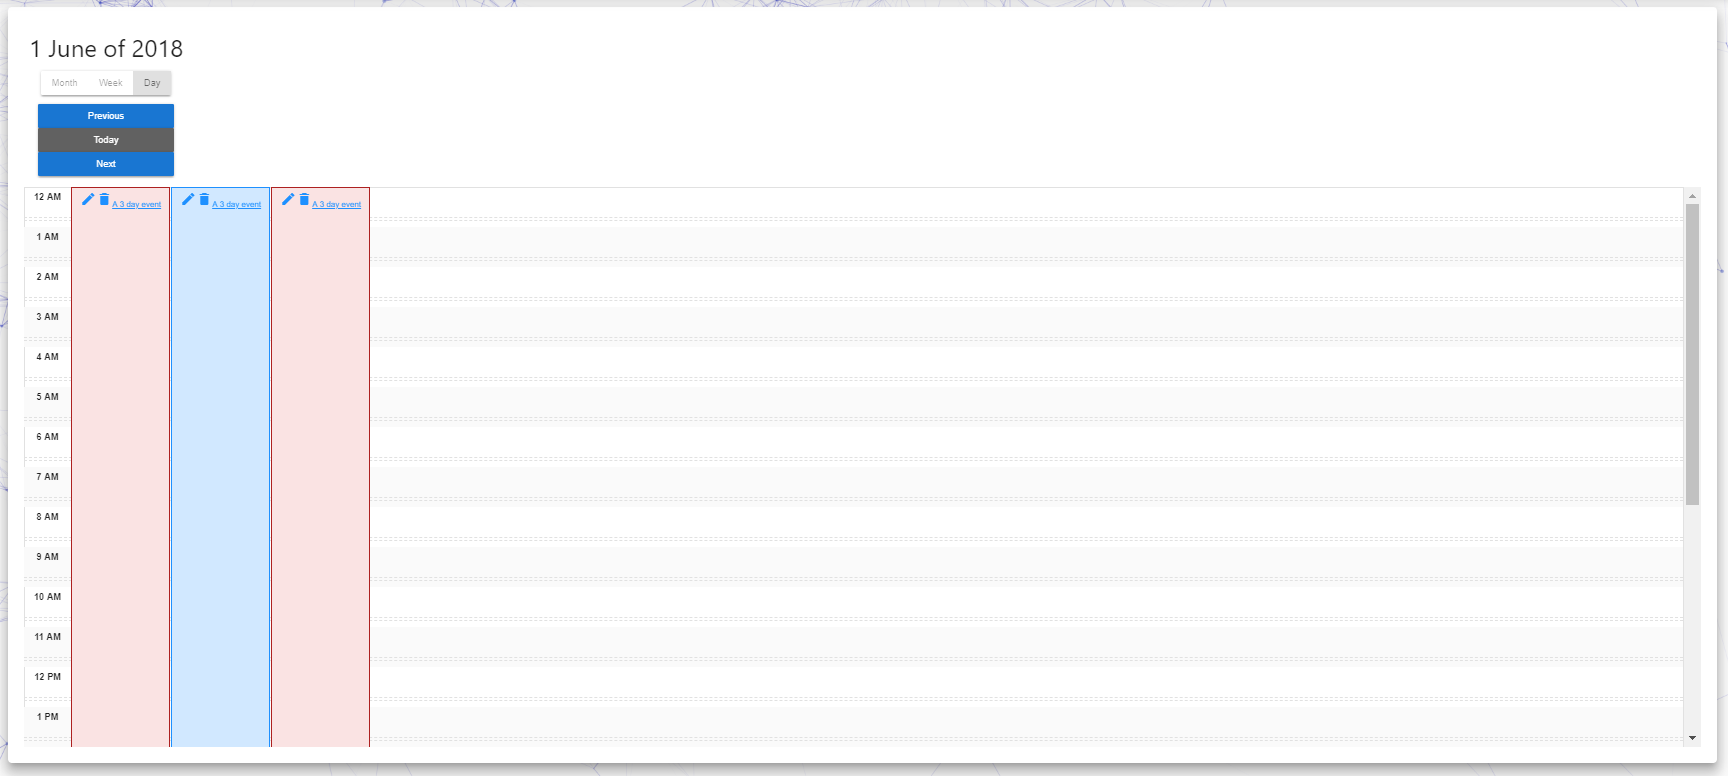
\includegraphics[width=\columnwidth, height=8cm]{images/userCalendarDay.png}
\caption{\e{User - Calendar Day}}
\label{fig:userCalendarDay}
\end{figure}

\pagebreak

\pSpace Για να προσθέσει ένα συμβάν στο ημερολόγιο, ο χρήστης πρέπει να επιλέξει την ημέρα που επιθυμεί, και ενεργοποιώντας το δεξί κλίκ επάνω της, εμφανίζεται ένα \e{Context Menu} με την επιλογή \e{Add Event}. Στην συνέχεια ανοίγει ένα \e{modal} παράθυρο (βλ. σχ. \ref{fig:userCalendarCreateEvent}).\\ \\
\pSpace Όπως και στην καρτέλα προφίλ, για ευκολότερη διαχείριση, χρησιμοποιήθηκαν \e{Expansion Panels}. Στην παρούσα περίπτωση, τρία \e{panels} συμπεριλαμβάνονται στο παράθυρο \e{Create Event}:\\
\begin{itemize}
	\item \e{Info} - Υπάρχουν δύο πεδία, κειμένου και \e{select}. Το πρώτο αφορά τον τίτλο του συμβάντος, ενώ το δεύτερο έχει ως επιλογές τα έργα του χρήστη. Με αυτόν τον τρόπο, σημειώνεται αν θα είναι προσωπικό συμβάν η κάποιου έργου.
	\item \e{Dates} - Δύο πεδία όπου ο χρήστης επιλέγει τις ημερομήνιες διεξαγωγής.
	\item \e{Type} - Ένα πεδίο \e{select} με τις επιλογές: \e{Danger, Info, Warning}. Ουσιαστικά εδώ ορίζει την κατηγορία στην οποία ανήκει, έτσι ώστε ο χρήστης να τα διακρίνει ευκολότερα. 
\end{itemize}

\begin{figure}[!htb]
\centering
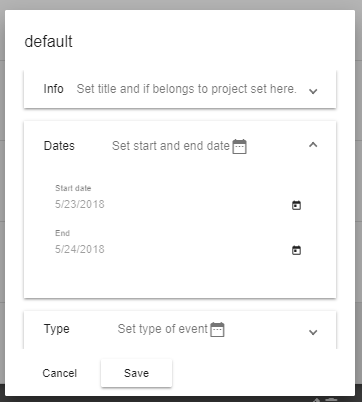
\includegraphics[scale=0.8]{images/userCalendarCreateEvent.png}
\caption{\e{User - Calendar Create Event}}
\label{fig:userCalendarCreateEvent}
\end{figure}

\pSpace Πίσω στο ημερολόγιο, έχοντας επιλεγμένη μια μέρα (οποιοδήποτε \e{view mode}), ο χρήστης έχει την δυνατότητα να σέρνει κάποιο σύμβαν προς άλλη μέρα, η ώρα, και εφόσον το αφήσει εκεί που επιθυμεί, αποθηκεύεται η επεξεργασία ημερομηνιών.\\
\pSpace Επιπλέον, για περαιτέρω επεξεργασία, επιλέγοντας κάποιο συμβάν εμφανίζεται το ίδιο παράθυρο όπως του σχ. \ref{fig:userCalendarCreateEvent}. Ακόμη, είτε στην περίπτωση δημιουργίας είτε επεξεργασίας, αν η πρώτη ημερομηνία είναι μεγαλύτερη της δεύτερης, εμφανίζεται σφάλμα με μια σύντομη περιγραφή, όπως και αν λείπει ο τίτλος. Αν δέν διορθωθεί δεν είναι επιτυχής η αποθήκευση.

\subsubsection*{\e{Chat}}
\pSpace Για να πετύχει το \e{Project Management}, επιβάλλεται να υπάρχει καλή επικοινωνία στην ομάδα. Το \e{iPM} προσφέρει την δυνατότητα αυτή, για να συζητήσουν τα μέλη μιας ομάδας κάποια θέματα.\\
\pSpace Η διεύθυνση \e{\url{https://pmthesis.herokuapp.com/app/chat}} φορτώνει στο πλαίσιο δεδομένων την καρτέλα του σχ. \ref{fig:userChat}.\\
\pSpace Η καρτέλα αποτελείται από:\\
\begin{itemize}
	\item Μενού με δυνατότητα απόκρυψης στα αριστερά.
	\item Γραμμη εργαλείων.
	\item Πλαίσιο συζήτησης.
	\item Γραμμη εργαλείων για αποστολή μηνύματος.
\end{itemize}

\pSpace Στο αριστερό μενού υπό τον υπότιτλο \e{Channels}, υπάρχει η λίστα έργων του χρήστη. Επιλέγοντας κάποιο από αυτά, θα εμφανίστουν όλα τα μηνύματα (βλ. σχ. \ref{fig:userChatMessage}) που ανήκουν στην συζήτηση του εν λόγω έργου, στο πλαίσιο συζήτησης. Σε αυτό το μενού, περιέχεται επίσης μια γραμμή εργαλείων, με ενέργειες που αφορούν την διαθεσιμότητα του χρήστη, αλλά και ρυθμίσεις για το \e{Chat}. Αυτές οι ρυθμίσεις προς το παρόν, δεν είναι διαθέσιμες.\\
\pagebreak
\pSpace Η γραμμή εργαλείων, πάνω απο το πλαίσιο συζήτησης, περιέχει έναν διακόπτη για την απόκρυψη του αριστερού μενού και τον τίτλο της συζήτησης, ο οποίος συμβαίνει να είναι ο τίτλος του έργου.\\
\pSpace Κάτω απο το πλαίσιο συζήτησης, παρατηρείται η γραμμή εργαλείων για την αποστολή μηνυμάτων στο τρέχων \e{channel thread}. Δεν υπάρχει περιορισμός χαρακτήρων για το μήνυμα που θα σταλθεί.\\

\begin{figure}[!htb]
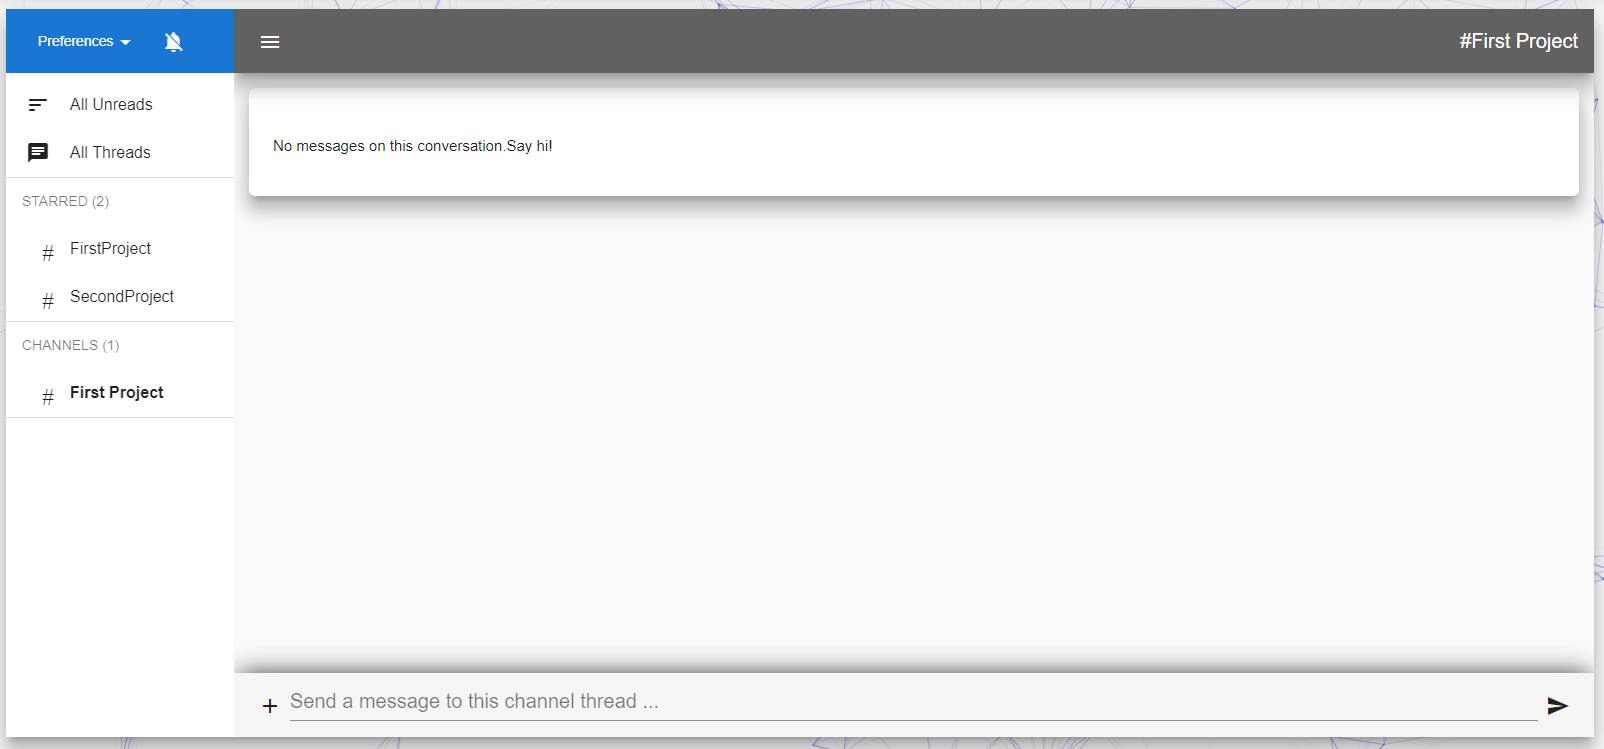
\includegraphics[width=\columnwidth, height=10cm]{images/userChat.png}
\caption{\e{User - Chat}}
\label{fig:userChat}
\end{figure}

\begin{figure}[!htb]
\centering

\includegraphics[width=\linewidth]{images/userChatMessage.png}
\caption{\e{User - Chat Message}}
\label{fig:userChatMessage}
\end{figure}

\subsubsection*{\e{Invites}}
\pSpace Για να συμβάλλει ένας χρήστης σε κάποιο έργο, θα χρειαστεί να τον προσκαλέσει κάποιο μέλος το έργου έν λόγω. Οι προσκλήσεις είναι διαθέσιμες στην διεύθυνση \e{\url{htts://pmthesis.herokuapp.com/app/invites}}, η οποία φορτώνει την καρτέλα του σχ. \ref{fig:userInvites}.\\
\pSpace Απεικονίζεται ένας πίνακας, στον οποίο οι εγγραφές έχουν την ακόλουθη μορφή: αριθμό, τίτλο έργου και 2 ενέργειες - αποδοχή και απόρριψη.

\begin{figure}[!htb]
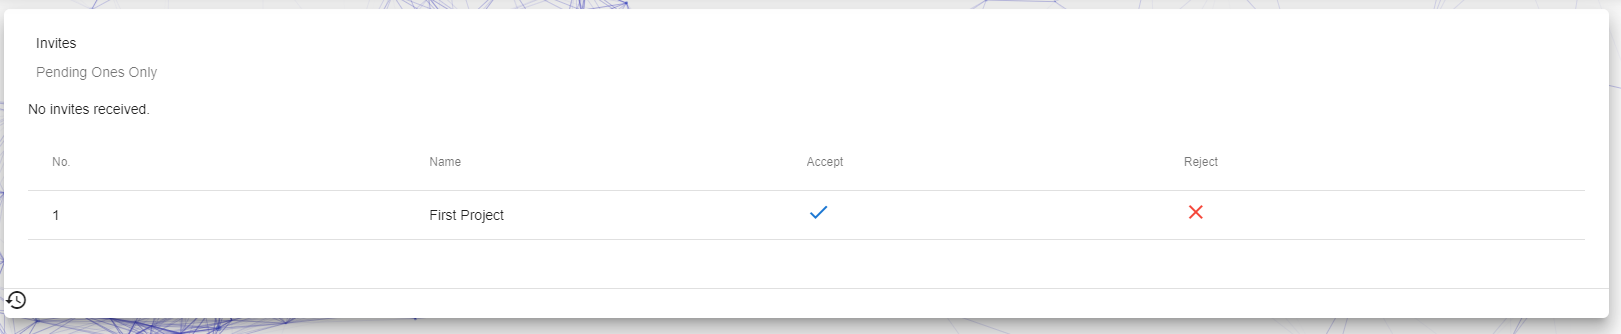
\includegraphics[width=\linewidth]{images/userInvite.png}
\caption{\e{User - Invites}}
\label{fig:userInvites}
\end{figure}

\subsubsection*{\e{404}}
\pSpace Κάποιες φορές είτε κατα λάθος, είτε σκόπιμα, ο χρήστης πληκτρολογεί μια διεύθυνση η οποία δεν υπάρχει. Για την αποφυγή προβλημάτων και σφαλμάτων, υπάρχει μια διεύθυνση, η οποία φορτώνεται αυτόματα όταν η διεύθυνση που πληκτρολογήθηκε είναι λανθασμένη. Ανακατευθύνει τον χρήστη στην διεύθυνση \e{\url{https://pmthesis.herokuapp.com/app/404}}. Σε αυτή την διεύθυνση φορτώνεται μια καρτέλα (βλ. σχ. \ref{fig:404}) στην οποία υπάρχει μια σύντομη περιγραφή του σφάλματος έτσι ώστε να μην ξανακάνει το ίδιο λάθος.

\begin{figure}[!htb]

\includegraphics[width=\linewidth]{images/404.png}
\caption{\e{404}}
\label{fig:404}
\end{figure}

% /User actions

\pagebreak

% Project actions
\subsection{\e{Project}}
\pSpace Στην ενότητα έργου, υπάρχουν δύο μέρη: το αριστερό μενού και η διεύθυνση. Το αριστερό μενού περιλαμβάνει τις ακόλυθες επιλογές:\\
\begin{itemize}
	\item \e{Dashboard}
	\item \e{Assignments}
	\item \e{Gantt}
	\item \e{Team}
	\item \e{Action Log}
	\item \e{Chat}
	\item \e{Settings}
\end{itemize}
\pSpace Όλες εξηγούνται παρακάτω, εκτός του \e{Chat}, το οποίο παραμένει ίδιο με αυτό που έχει αναφερθεί ήδη στην ενότητα \e{User}.\\
\pSpace Επίσης, σημειώνεται πως όλα τα δεδομένα πλέον αφορούν το έργο.

\subsubsection*{\e{Dashboard}}
\pSpace Ανοίγωντας κάποιο έργο, ο χρήστης θα συναντήσει πρώτα το \e{Dashboard} (βλ. σχ. \ref{fig:projectDashboard}) στην διεύθυνση \e{\url{https://pmthesis.herokuapp.com/app/project/dashboard}}. Εδώ φορτώνονται τέσσερις καρτέλες (δύο είναι μη διαθέσιμες προς το παρόν). Οι δύο που είναι ενεργές, έχουν τον ίδιο σχεδιασμό και λειτουγία, αλλα διαφορετικά δεδομένα:
\begin{itemize}
	\item Η πρώτη καρτέλα δείχνει τα στατιστικά για τα \e{Tasks}.
	\item Η δεύτερη απεικονίζει τα στατιστικά για τα \e{Issues}.
\end{itemize}

\begin{figure}[!htb]
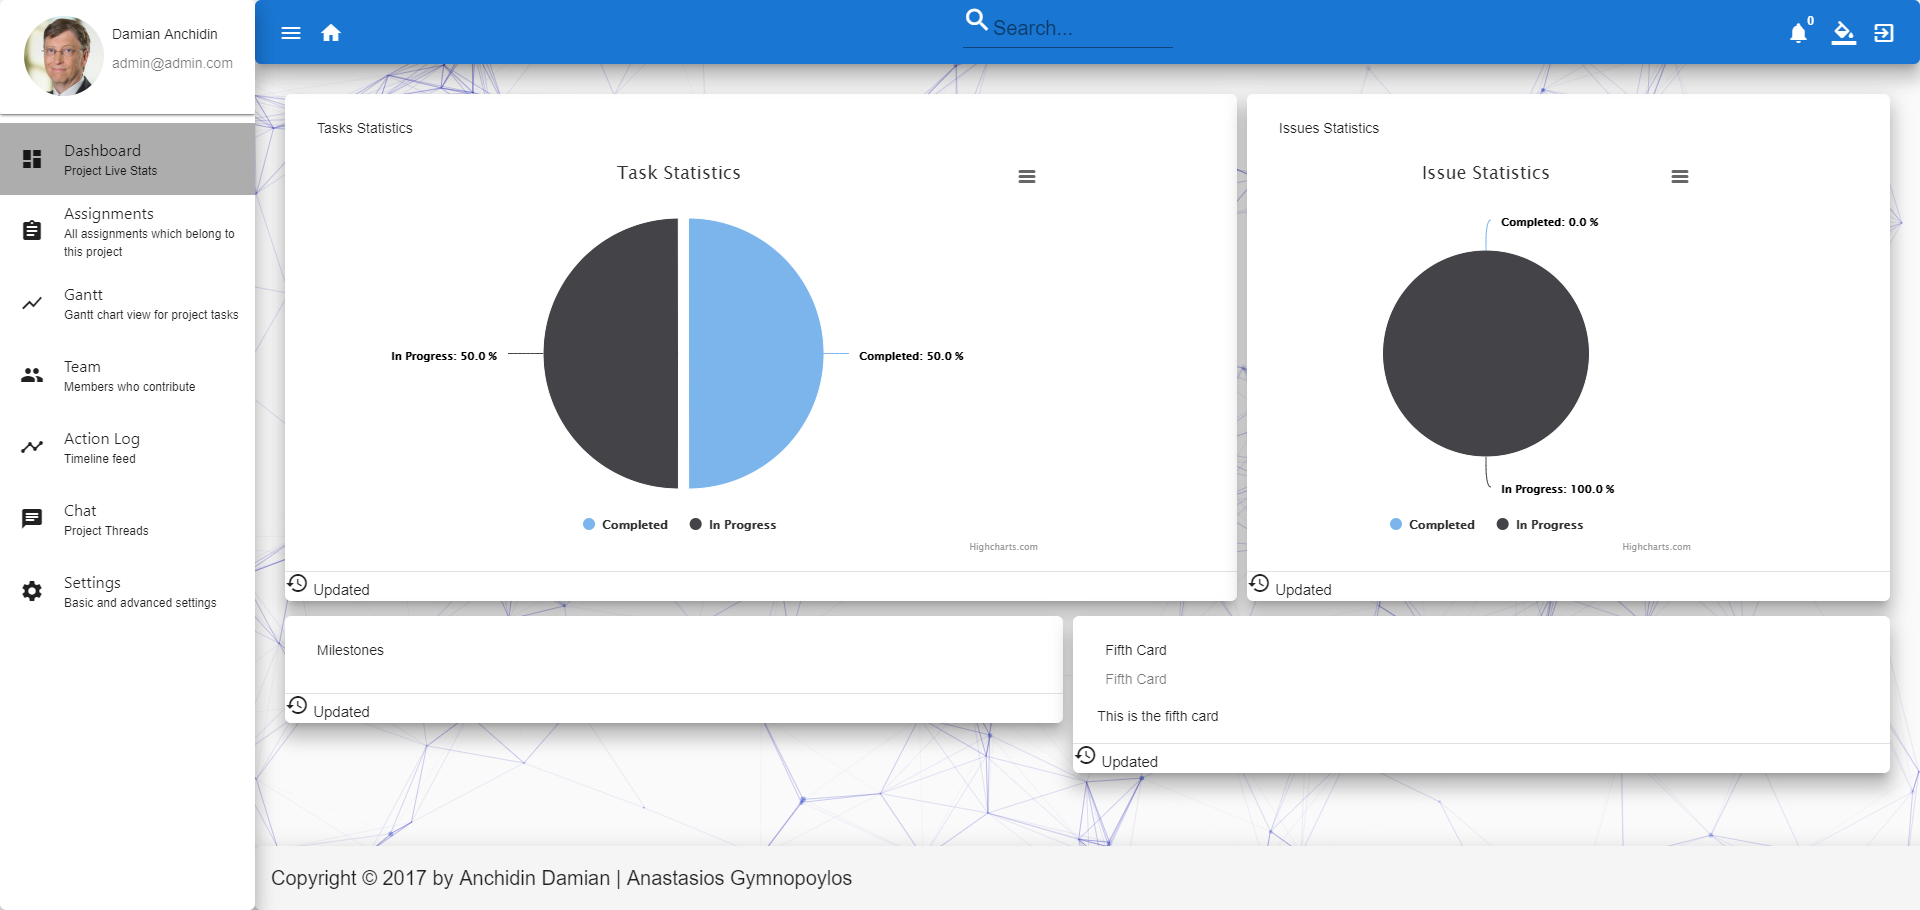
\includegraphics[width=\linewidth]{images/projectDashboard.png}
\caption{\e{Project - Dashboard}}
\label{fig:projectDashboard}
\end{figure}

\pSpace Και στις δύο περιπτώσεις, χρησιμοποιήθηκαν διαγράμματα σε μορφή πίτας (\e{Pie Chart}). Όπως όλα τα διαγράμματα της εφαρμογής, προσφέρουν την δυνατότητα εκτύπωσης και κατεβάσματος. Επιπλέον, σε περίπτωση που δεν υπάρχουν δεδομένα, το διάγραμμα εξαφανίζεται, και μένει μια συντόμευση που οδηγεί τον χρήστη στην δημιουργία \e{Tasks} και \e{Issues}.

\pagebreak

\subsubsection*{\e{Assignments}}
\pSpace Η ανάθεση εργασιών στα μέλη του έργου, είναι μια απο τις βασικότερες έννοιες του \e{Project Management}. Στην εφαρμογή \e{iPM} αυτό αλλά και η διαχείρισή τους επιτυγχάνεται από την επιλογή \e{Assignments} του αριστερού μενού, που αδηγεί στην διεύθυνση \e{\url{https://pmthesis.herokuapp.com/app/project/assignments}}. Εδώ φορτώνεται μια καρτέλα η οποία είναι η βάση για το υπόλοιπα (βλ. σχ. \ref{fig:projectAssignments}).

\begin{figure}[!htb]
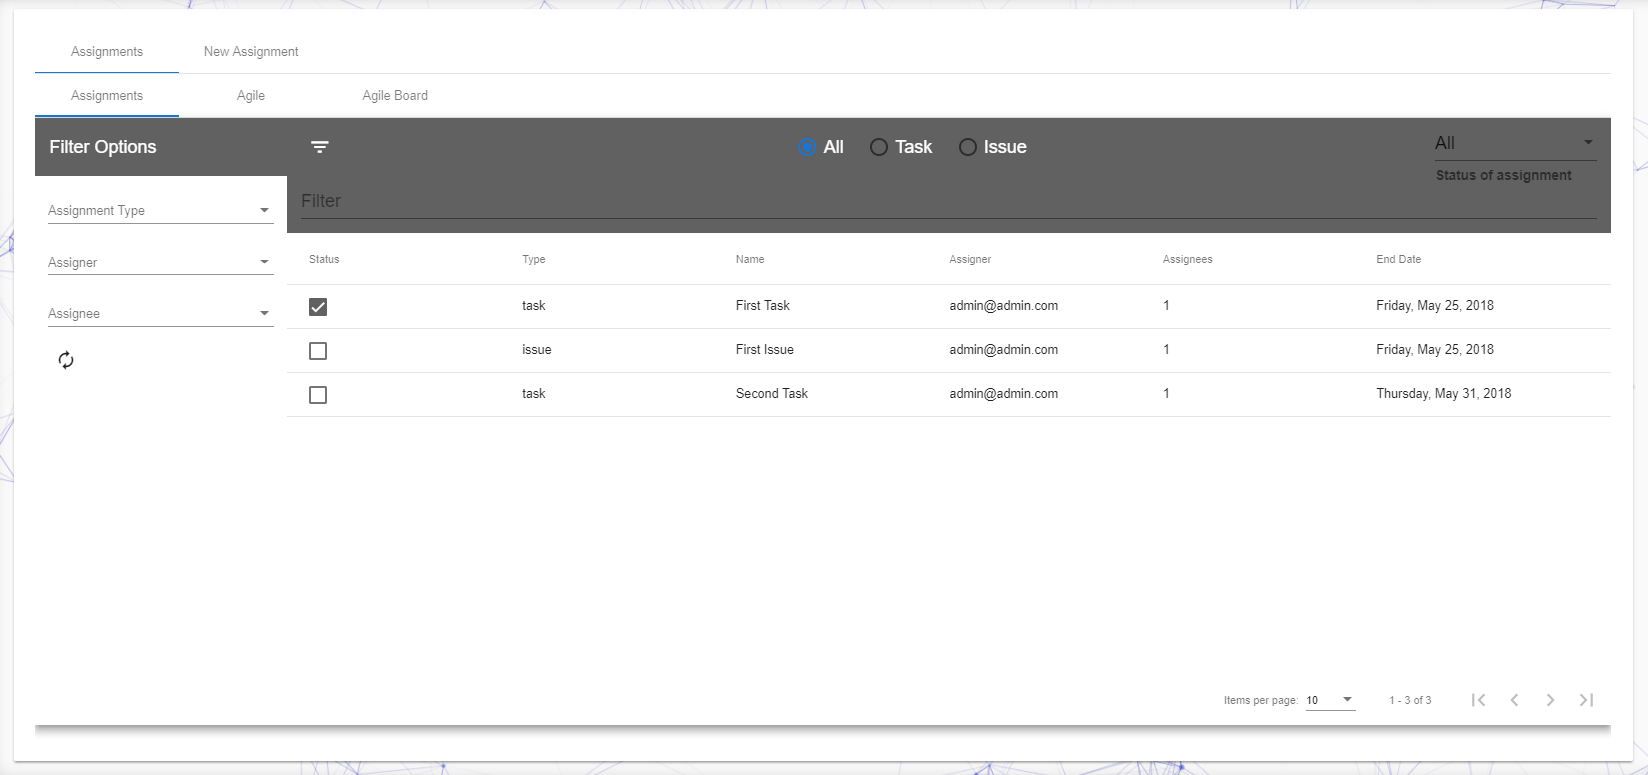
\includegraphics[width=\linewidth, height=8cm]{images/projectAssignments.png}
\caption{\e{Project - Assignments landing}}
\label{fig:projectAssignments}
\end{figure}

\pSpace Όπως φαίνεται και απο το σχ. \ref{fig:projectAssignments}, υπάρχουν στον επάνω μέρος της καρτέλας δύο \e{tab}: \e{Assignments} και \e{New Assignment}. Θα εξηγήσουμε αρχικά το πρώτο.\\
\pSpace Στο πρώτο λοιπόν, περιλαμβάνονται άλλα τρία \e{tab} τα οποία φορτώνονται σε άλλη διεύθυνση σε σχέση με τα \e{tab} που υπήρχαν στην εφαρμογή. Το πρώτο στην σειρά αφορά μια κλασική απεικόνιση των εργασιών (βλ. σχ. \ref{fig:projectAssignmentsAssignments}), δηλαδή έναν πίνακα όπου η κάθε εγγραφή εκπροσωπεύει ένα \e{task} η \e{issue}. Η διεύθυνση αυτού είναι \e{\url{https://pmthesis.herokuapp.com/app/project/assignments/(assignments:assignments)}}.\\
\pSpace Μια εγγραφή αποτελείται από την κατάσταση της εργασίας, ολοκληρωμενή η μή, ο τύπος (\e{Task, Issue}), τίτλος, ο χρήστης που την δημιούργησε, το σύνολο των μέλων στους οποίους ανατέθηκε αύτη η εργασία και η ημερομηνία στην οποία θα πρέπει να έχει ήδη ολοκληρωθεί.\\
\pSpace Η κατάσταση της εργασίας μπορεί να αλλάξει ενεργοποιώντας το \e{check box} που φαίνεται στην πρώτη στήλη, εφόσον ο χρήστης έχει πρόσβαση, δηλαδή να είναι δημιουργός η να ανήκει στην ομάδα που το έχει αναλάβει.\\
\pSpace Επιλέγοντας μια εργασία, δηλαδή ενεργοποιώντας το κλίκ πάνω στην εγγραφή (εκτός \e{checkbox}), ανακατευθύνει τον χρήστη στην αναλυτική όψη. \pSpace Πάνω από τον πίνακα, παρατηρείται μια ομάδα από κουμπιά τύπου \e{radio}, ένα πεδίο \e{select} και ένα πεδίο κειμένου, τα οποία εκπληρώνουν την λειτουργία του φιλτραρίσματος. Τα φίλτρα που αναφέραμε, εφαρμόζονται ταυτοχρόνος, δηλαδή το αποτέλεσμα επηρεάζεται απο το σύνολο τους.\\
\pSpace Επιπλέον, στο αριστερό μέρος του πίνακα υπάρχει ένα μενού (επίσης με δυνατότητα απόκρυψης), στο οποίο βρίσκονται άλλα φίλτρα πιο συγκεκριμένα, προς το παρόν όμως δεν έιναι διαθέσιμα.\\
\pSpace Ο πίνακας διαθέτει σελιδοποιήση και ρύθμιση των εγγραφών ανά σελίδα.

\begin{figure}[!htb]
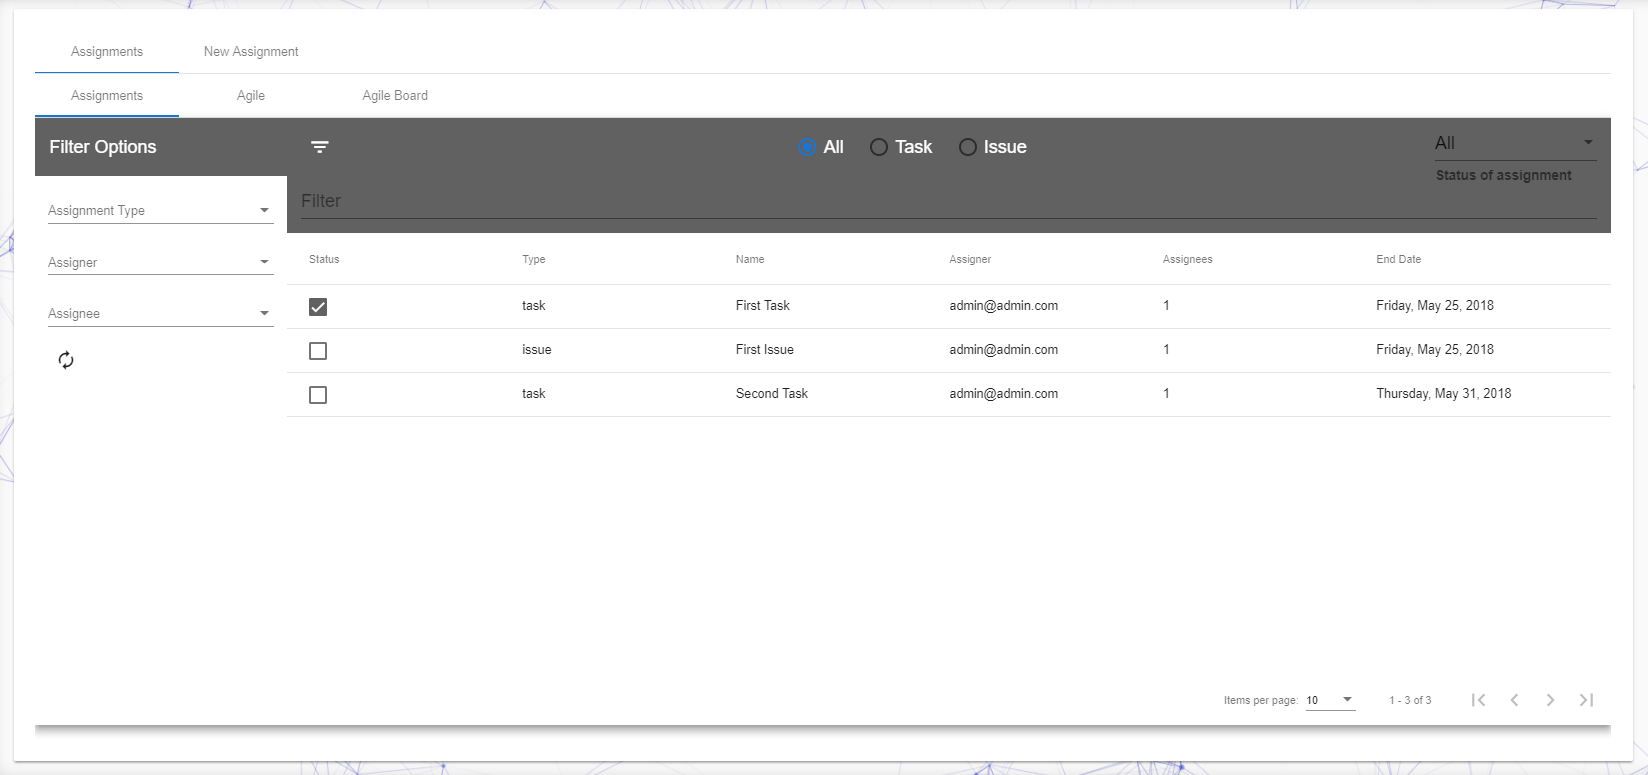
\includegraphics[width=\linewidth, height=8cm]{images/projectAssignmentsAssignments.png}
\caption{\e{Project - Assignments Classic}}
\label{fig:projectAssignmentsAssignments}
\end{figure}

\pSpace Τα επόμενα δύο \e{tab}, δέν είναι διαθέσιμα προς το παρόν.\\

\pSpace Το \e{tab} με τίτλο \e{Create Assignment} (βλ. σχ. \ref{fig:projectCreateAssignment}) εξυπηρετεί την δημιουργία νέας εργασίας. Αποτελείται από τέσσερα \e{Expansion Panels} για να διευκολύνει την χρήση. Τα \e{panels} πηγαίνουν ως εξής:\\

\begin{itemize}
	\item Στο πρώτο εισάγονται τα βασικά στοιχεία όπως τύπος, τίτλος και μια σύντομη περιγραφή (2048 χαρακτήρες μέγιστο).
	\item Στο δεύτερο εισάγεται το εύρος ημερομηνιών.
	\item Το τρίτο αφορά τα άτομα στα οποία θα ανατεθεί η εν λόγω εργασία. Ο χρήστης μπορεί να πληκτρολογήσει τις ηλεκτρονικές διευθύνσεις ή να επιλέξει από το αύτα που εμφανίζονται. Το συγκεκριμένο πεδίο είναι τύπου \e{select} αλλά και εισαγωγή κειμένου. Χωρίζοντας τις διευθύνσει με κόμμα, τις προσθέτει κατευθείαν στην λίστα.
	\item Το τελευταίο αφορά τις εξαρτήσεις. Αν επιλέξει να ορίσει κάποια η πολλαπλές εξαρτήσεις, θα ανοίξει ένα \e{modal} παράθυρο που περιέχει έναν πίνακα με τις υπαρκτές εργασίες και τον τύπο εξάρτησης.
\end{itemize}

\begin{figure}[!htb]
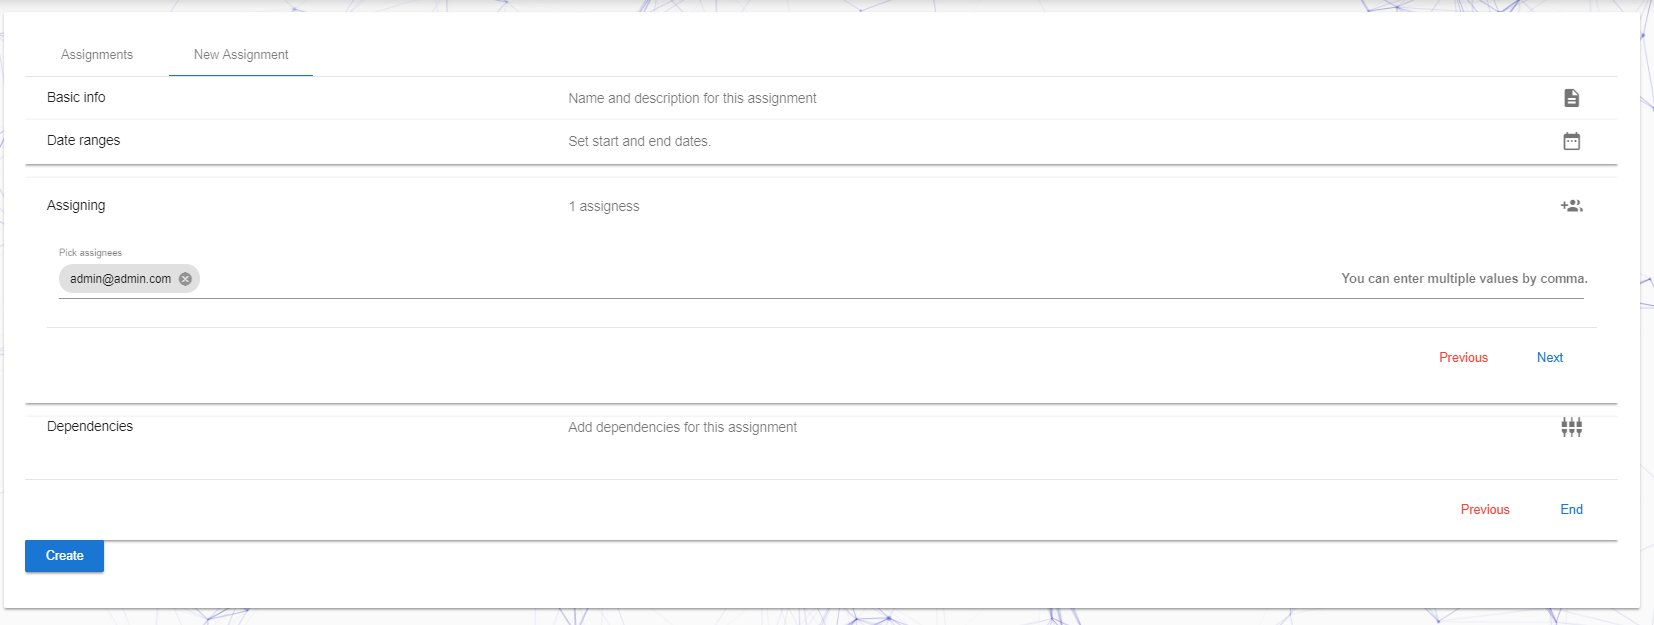
\includegraphics[width=\linewidth, height=8cm]{images/projectCreateAssignment.png}
\caption{\e{Project - Create Assignment}}
\label{fig:projectCreateAssignment}
\end{figure}

\pSpace Επιλέγοντας κάποια εργασία, ανακατευθύνει τον χρήστη στην διεύθυνση \e{\url{https://pmthesis.herokuapp.com/app/assignmentview/@id}} η οποία φορτώνει 2 καρτέλες, μια σχεδόν ίδια με το σχ. \ref{fig:projectCreateAssignment} και μια για τα σχόλια της έν λόγω εργασία. Η δεύτερη δεν είναι ακόμη διαθέσιμη.\\
\pSpace Η πρώτη καρτέλα έχει επιπλέον την κατάσταση της εργασίας ως διαφορές στο σχεδιασμό. Όμως, αν ο χρήστης επιθυμεί να την επεξεργαστεί, θα πρέπει να είναι είτε ο δημιουργός, είτε να ανήκει στην ομάδα που την έχει αναλάβει, αλλιώς όλα τα πεδία είναι απενεργοποιημένα.

\begin{figure}[!htb]
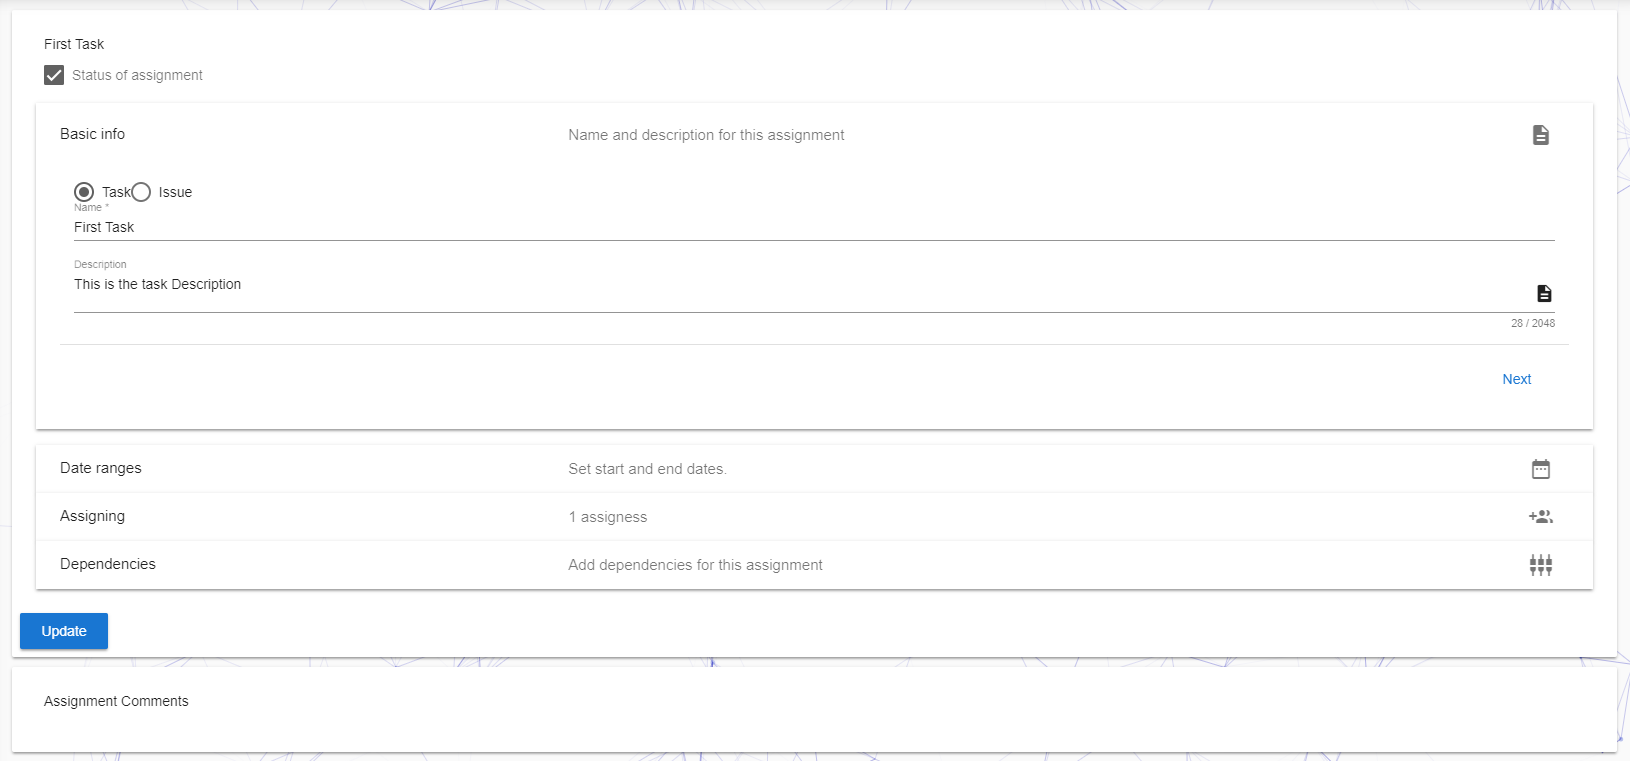
\includegraphics[width=\linewidth, height=8cm]{images/projectAssignementView.png}
\caption{\e{Project - Assignment View$\&$Edit}}
\label{fig:projectAssignmentView}
\end{figure}

\pagebreak

\subsubsection*{\e{Gantt}}
\pSpace Η διεύθυνση \e{\url{https://pmthesis.herokuapp.com/app/project/gantt}} φορτώνει την καρτέλα με το διάγραμμα Γκάνττ. Το διάγραμμα είναι ίδιο με αυτό που βρίσκεται στην ενότητα \e{User}, με την διαφορά ότι τα δεδομένα που προβάλλονται ανήκουν στο έργο και είναι μόνο τύπου \e{Task}. Οι εργασίες που έχουν κάποιου έιδους εξάρτηση μεταξύ τους είναι ομαδοποιημένα, και σχετίζονται με βελάκια που παριστάνουν την εξάρτηση.

\begin{figure}[!htb]
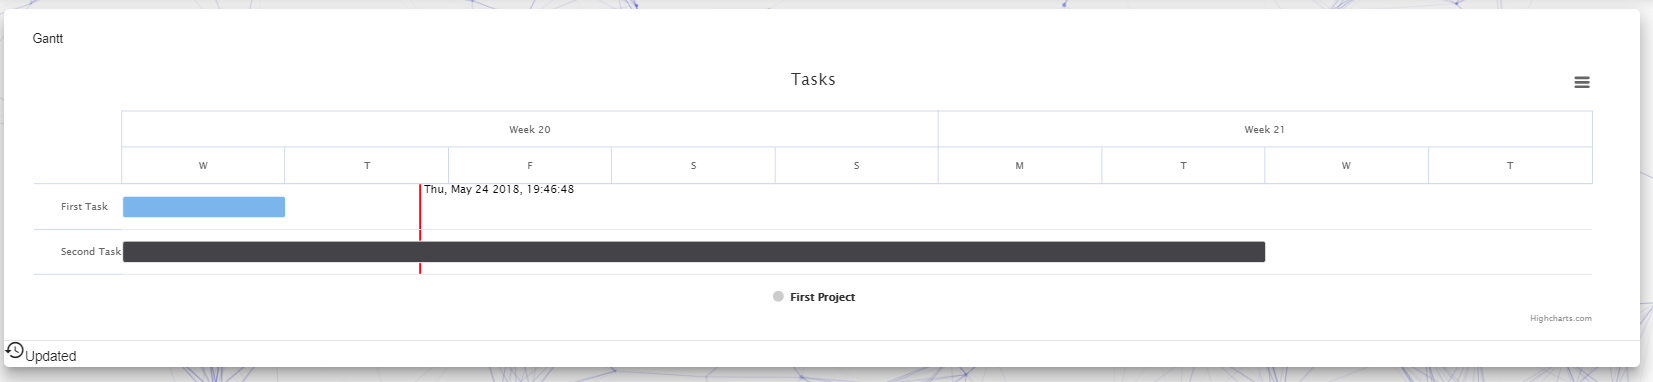
\includegraphics[width=\linewidth, height=6cm]{images/projectGantt.png}
\caption{\e{Project - Gantt}}
\label{fig:projectGantt}
\end{figure}

\subsubsection*{\e{Team}}
\pSpace Η επόμενη επιλογή στο αριστερό μενού, στην ενότητα έργου, είναι το \e{Team}, με διεύθυνση \e{\url{https://pmthesis.herokuapp.com/app/project/team}}. Φορτώνει στο πλαίσιο δεδομένων δύο καρτέλες (βλ. σχ. \ref{fig:projectTeam}).\\
\pSpace Στην πρώτη καρτέλα, απεικονίζεται η ομάδα του έργου σε μορφή πίνακα. Κάθε εγγραφή παριστάνωντας ένα μέλος με τις ακόλουθες πληροφορίες: αριθμός, ηλεκτρονική διεύθυνση, ρόλος. Σε κάθε εγγραφή, δίνεται η δυνατότητα αφαίρεσης της, και έμμεσα του μέλους από την ομάδα.\\
\pSpace Στην δεύτερη καρτέλα υπάρχει ένα πεδίο κειμένου, όπως αυτό στην δημιουργία έργου, όπου πληκτρολογεί ο χρήστης τα άτομα που επιθυμεί να προσκαλέσει στην ομάδα.

\begin{figure}[!htb]
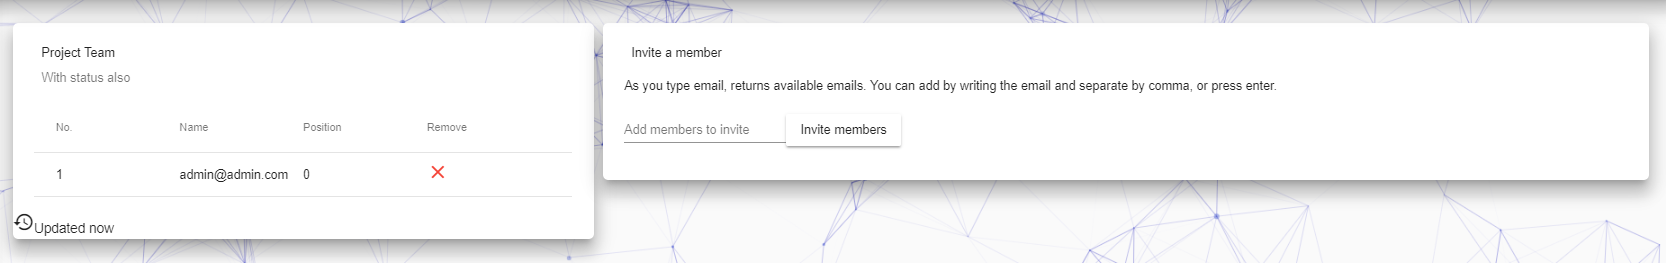
\includegraphics[width=\linewidth]{images/projectTeam.png}
\caption{\e{Project - Team}}
\label{fig:projectTeam}
\end{figure}

\subsubsection*{\e{Action Log}}
\pSpace Το \e{Action Log} αναφέρεται στο χρονοδιάγραμμα έργου, όπου σημειώνονται τα σημαντικότερα σύμβαντα. Βρίσκεται στην διεύθυνση \e{\url{https://pmthesis.herokuapp.com/app/project/timeline}} και φορτώνει την καρτέλα του σχ. \ref{fig:projectTimeline}.\\
\pSpace Η σειρά των εγγραφών είναι με βάση τις ημερομηνίες τους. Επιλέγοντας κάποια εγγραφή του χρονοδιαγράμματος, εμφανίζει κάτω από την ίδια περαιτέρω πληροφορίες σχετικά με αυτήν.

\begin{figure}[!htb]
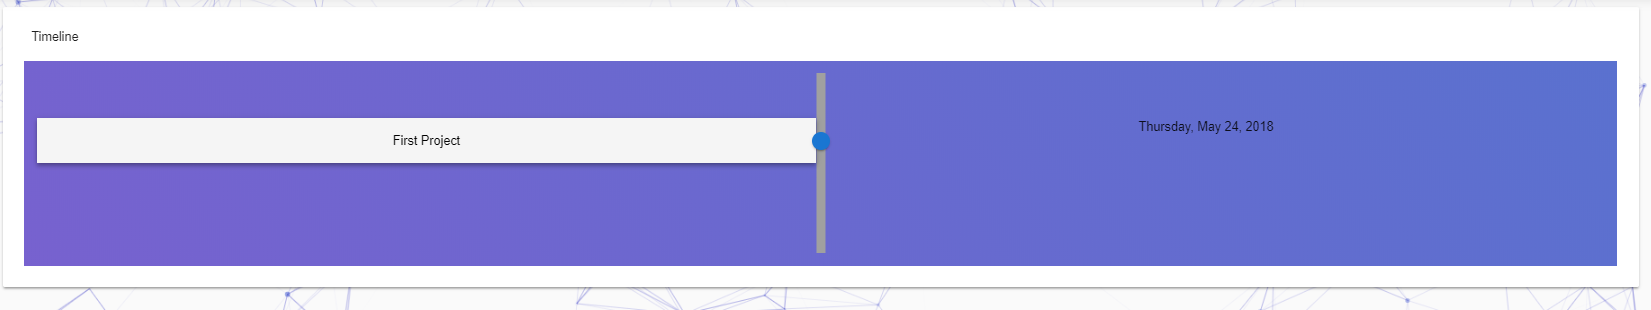
\includegraphics[width=\linewidth]{images/projectTimeline.png}
\caption{\e{Project - Action Log}}
\label{fig:projectTimeline}
\end{figure}

\subsubsection*{\e{Settings}}
\pSpace Τελευταία επιλογή του μενού, πηγαίνει τον χρήστη στις ρυθμίσεις έργου, οι οποίες έιναι προσβάσιμες άν ο χρήστης έιναι ο διαχειριστής, αλλιώς τον ανακατευθύνει στο \e{Dashboard} του έργου. Η διεύθυνση \e{\url{https://pmthesis.herokuapp.com/app/project/settings}} φορτώνει στον πλαίσιο δεδομένων δύο καρτέλες (βλ. σχ. \ref{fig:projectSettings}). Και οι δύο αποτελούνται από τέσσερα \e{Expansion Panels}.\\
\pSpace Η πρώτη καρτέλα, αφορά τα βασικά στοιχεία του έργου τα οποία εισάχθηκαν στην δημιουργία:\\
\begin{itemize}
	\item Εταιρία
	\item Τίτλος
	\item Προυπολογισμός
	\item Σύντομη περιγραφή
\end{itemize}

\pSpace Η δεύτερη καρτέλα αφορά ρυθμίσεις που χρειάζονται την προσοχή του διαχειριστή:\\

\begin{itemize}
	\item \e{Privacy} - Αν το έργο είναι ιδιωτικό η δημόσιο. Αυτό επηρεάζει τα αποτελέσματα αναζήτησης.
	\item Ιδιοκτησία - Εδώ ο διαχειριστής, μπορεί να δώσει τον ρόλο του σε άλλο μέλος του έργου.
	\item Κλείδωση - Αν αποφασίσει να κλειδώσει το έργο ο διαχειριστής, σημαίνει πώς δεν μπορούν να λάβουν θέση άλλες ενέργειες, παρά μόνο προβολή των πληροφοριών.
	\item Διαγραφή - Διαγραφή έργου και όλως των δεδομένων (\e{Task, Issue} κλπ)
\end{itemize}

\pSpace Το κουμπί στο δεξιό μέρος του πλαισίου δεδομένων έχει τον ρόλο αποθήκευσης αλλαγών.

\begin{figure}[!htb]
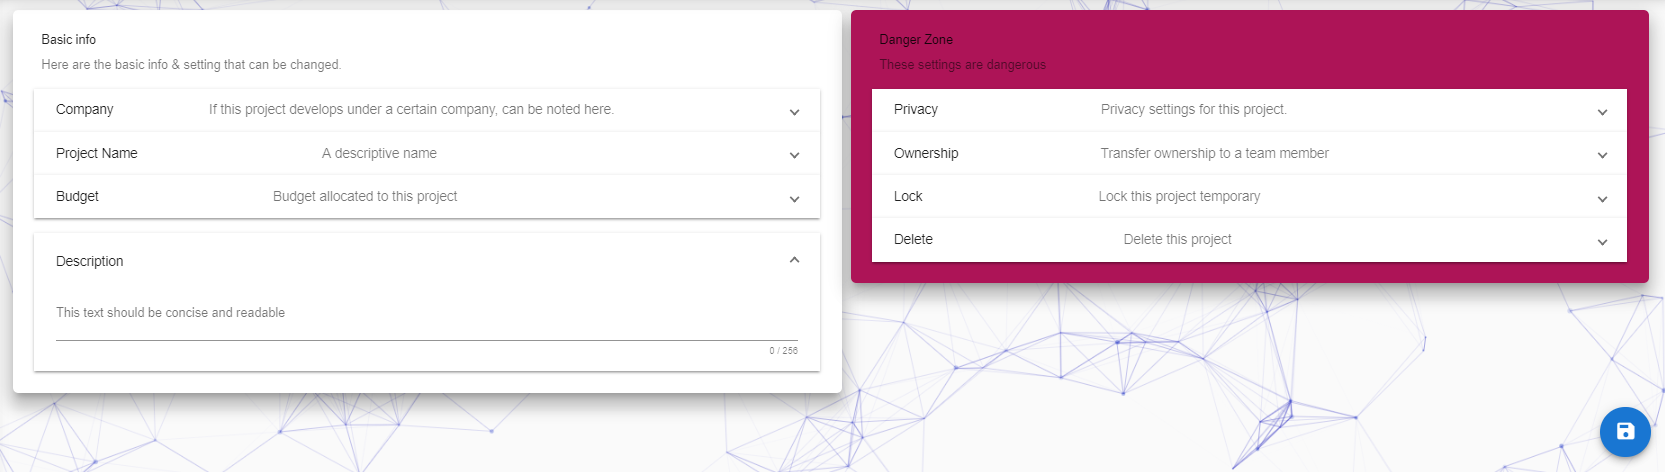
\includegraphics[width=\linewidth]{images/projectSettings.png}
\caption{\e{Project - Settings}}
\label{fig:projectSettings}
\end{figure}

\subsubsection*{\e{Notifications}}
\pSpace Οι ειδοποιήσεις είναι τύπου \e{Push} (βλ. σχ. \ref{fig:pushNotification}), και χρειάζονται την αποδοχή του χρήστη για να εμφανιστούν. Περιέχουν τίτλο, περιγραφή και σε μερικές περιπτώσεις συνδέσμους για γρήγορα πρόσβαση στις υπόλοιπες πληροφορίες.\\
\pSpace Επιπλέον, το σύνολο ειδοποιήσεων φαίνεται ενεργοποιώντας τον διακόπτη για το δεξιό μενού, απο την πάνω γραμμή εργαλειών. Αυτό ανοίγει τα \e{Notifications} ομαδοποιημένα σε δύο κατηγορίες: \e{Seen, Unseen} (βλ. σχ. \ref{fig:userNotifications}).

\begin{figure}[!htb]
\centering

\includegraphics[scale=0.5]{images/pushNotification.png}
\caption{\e{Notification}}
\label{fig:pushNotification}
\end{figure}

\begin{figure}[!htb]
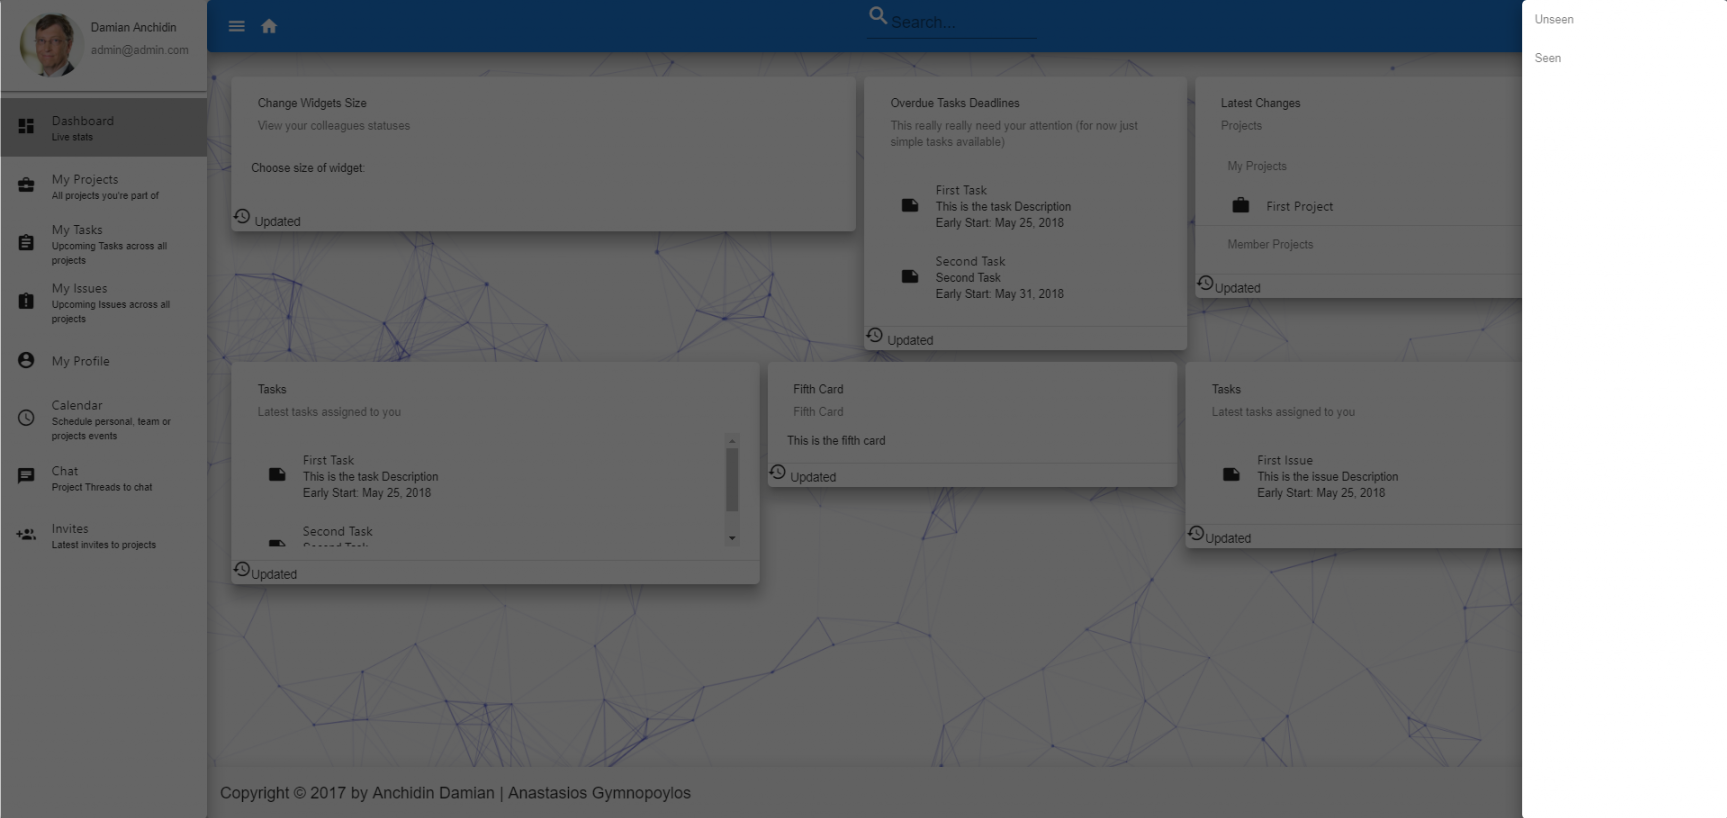
\includegraphics[width=\linewidth]{images/userNotifications.png}
\caption{\e{Notifications}}
\label{fig:userNotifications}
\end{figure}

\subsubsection*{\e{Theme}}
\pSpace Το κουμπί για το θέμα σχεδιασμού που βρίσκεται στην πάνω γραμμή εργαλειών, ανοίγει ένα \e{Context Menu} με τέσσερις επιλογές (δύο διαθέσιμες). Η μια είναι η προκαθορισμένη, ενώ η δεύτερη φαίνεται στο σχ. \ref{fig:userDashboardDark}.

\begin{figure}[!htb]
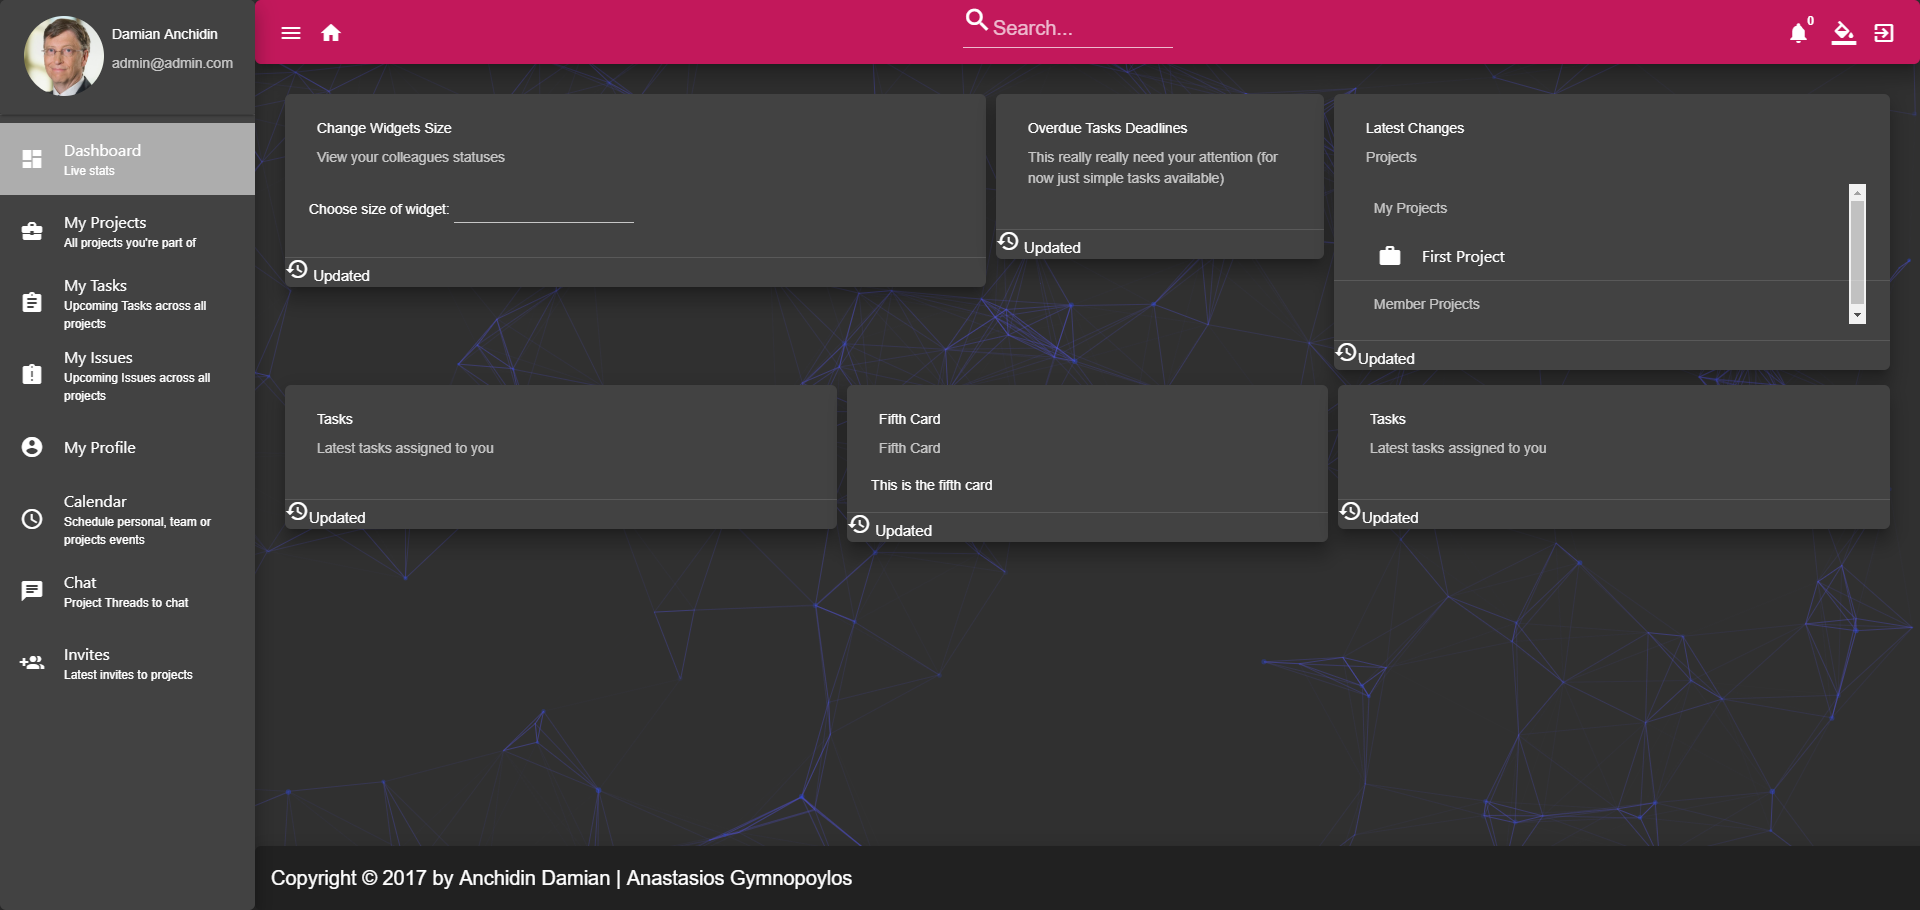
\includegraphics[width=\linewidth]{images/userDashboardTHEME2.png}
\caption{\e{Dark Theme}}
\label{fig:userDashboardDark}
\end{figure}

% /Project actions